\documentclass[11pt]{article}
\usepackage{amsmath, amsthm, amssymb, pdfpages} 
\usepackage{fullpage}
\usepackage{hyperref}
\usepackage{graphicx}
\usepackage[capitalize]{cleveref}
\usepackage[CaptionBefore]{fltpage} % for large figures, captions go on prev page

% options for pretty tables from CSV files
\usepackage{booktabs,csvsimple,siunitx}
% for commas in big numbers (i.e. "3,000,000")
\sisetup{group-separator={,}}

% next three for UTF8 to work (for non-ASCII names to work without awkward codes)
\usepackage[T1]{fontenc}
\usepackage{textcomp}
\usepackage[utf8]{inputenc}

% import biblatex with prefered settings
% loads biblatex with all the nice standard options that John determined some time ago!
% this version uses a ``Harvard'' style (first author last name, year in parentheses).
% also loads xpatch

% biblatex
% harvard style
\usepackage[style=authoryear,natbib,maxcitenames=2,doi=false,isbn=false,url=false,backend=bibtex]{biblatex}
% numeric style
%% \usepackage[style=numeric-comp,sorting=none,giveninits=true,
%%                      doi=false,isbn=false,url=false,backend=bibtex]{biblatex}
% remove "In: " before journal title
\renewbibmacro{in:}{}
% remove language
\AtEveryBibitem{\clearlist{language}}
% remove month
\AtEveryBibitem{\clearfield{month}}
% and also notes
\AtEveryBibitem{\clearfield{note}}
% remove dots between volume and issue
\usepackage{xpatch}
\xpatchbibmacro{volume+number+eid}{%
  \setunit*{\adddot}%
}{%
}{}{}
% put issue in parentheses
\DeclareFieldFormat[article]{number}{\mkbibparens{#1}}


\bibliography{zotero, dummy}

% path of images
\graphicspath{ {../data/} }

% define shortcuts for awkward math symbols
% this also helps us change them more easily later, if needed
\newcommand{\rmsd}{\text{SRMSD}_p}
\newcommand{\auc}{\text{AUC}_\text{PR}}

\usepackage{kinshipsymbols}

% double line spacing (PLoS wants this)
\usepackage{setspace}
\doublespacing
% original, smaller spacing
%\renewcommand{\baselinestretch}{1.2}

% cool automatic supplemental figures/tables!
% http://bytesizebio.net/2013/03/11/adding-supplementary-tables-and-figures-in-latex/
% with some additions
\newcommand{\beginsupplement}{%
  \setcounter{table}{0}
  \renewcommand{\thetable}{S\arabic{table}}%
  \setcounter{figure}{0}
  \renewcommand{\thefigure}{S\arabic{figure}}%
  \setcounter{section}{0}
  \renewcommand{\thesection}{S\arabic{section}}%
  \setcounter{equation}{0}
  \renewcommand{\theequation}{S\arabic{equation}}%
  \setcounter{page}{1}
  \renewcommand{\thepage}{S\arabic{page}}%
}


% OLD: Testing the effectiveness of principal components in adjusting for relatedness in genetic association studies
\title{\Large \textbf{
    Limitations of principal components in quantitative genetic association models for human studies
  }}
\author{Yiqi Yao$^1$, Alejandro Ochoa$^{1,2,*}$}
\date{}

\begin{document}
\maketitle

\noindent
$^1$ Department of Biostatistics and Bioinformatics, Duke University, Durham, NC 27705, USA \\
$^2$ Duke Center for Statistical Genetics and Genomics, Duke University, Durham, NC 27705, USA \\
$^*$ Corresponding author: \texttt{alejandro.ochoa@duke.edu}

\begin{abstract}
  Modern genetic association studies require modeling population structure and family relatedness in order to calculate correct association statistics.
  Principal Components Analysis (PCA) is an efficient, flexible, and one of the most common models for population structure, but nowadays the Linear Mixed-Effects Model (LMM) is believed by many to be a superior association model.
  % might change depending on lit search
  Remarkably, previous PCA evaluations have been limited, for example, by not varying the number of principal components (PCs), by simulating unrealistically simple population structures, and not using real genotype data.
  The use of LMMs with PCs has also been proposed, but evidence of effectiveness is lacking.
  In this work, we thoroughly evaluate PCA and LMM both with varying number of PCs in various realistic genotype and complex trait simulation scenarios, including admixture together with family structure, large real multiethnic human datasets (1000 Genomes Project, the Human Genome Diversity Panel, and Human Origins), and simulations from trees fit to each real dataset.
  We find that LMM without PCs performs best in all cases, with the largest effects in the family simulation and all of the real human datasets.
  We determined that the large gaps in PCA to LMM performance on the real human datasets is due to the high-dimensional family structure from large numbers of distant relatives, and not from the smaller number of highly related individuals present.
  While it was known that PCA fails on family data, here we report a strong effect on association of cryptic family relatedness in several human datasets that focused on capturing genetic diversity.
  Overall, this work better characterizes the limitations of principal components compared to mixed effects models in modeling the complex relatedness structures present in simulated and real multiethnic human data.

  % used for ASHG abstract
  %\textbf{Keywords:} genetic association, statistical genetics, population structure, complex traits, genetic diversity.
\end{abstract}

% \clearpage

% \tableofcontents

%\section{Author Summary}
% TODO: PLoS specific section
% https://journals.plos.org/plosgenetics/s/submission-guidelines

\section{Introduction} 

% need for specialized approaches
The goal of a genetic association study is to identify loci whose genotype variation is significantly correlated to given trait.
An important, implicit assumption made by classical association tests is that, under the null hypothesis, genotypes are unstructured: drawn independently from a common allele frequency.
However, this assumption does not hold for structured populations, which includes multiethnic cohorts and admixed individuals, and for family data.
When naive approaches are incorrectly applied to structured populations or family data, association statistics (such as chi-squared) become inflated relative to the null expectation, resulting in greater numbers of false positives than expected and loss of power \citep{devlin_genomic_1999, voight_confounding_2005, astle_population_2009}.
Therefore, many specialized approaches have been developed for genetic association in structured data.
Here we focus on extensively evaluating the two most popular association models: principal components analysis (PCA) and linear mixed-effects models (LMM).

% PCA
Many association models for structured populations are generalized linear models that incorporate this structure via covariates, which have included inferred ancestry or admixture proportions \citep{pritchard_association_2000} or transformations of these.
PCA represents the most common of these variants nowadays, in which the top eigenvectors of the population kinship matrix are used to model the population structure \citep{zhang_semiparametric_2003, price_principal_2006, bouaziz_accounting_2011}.
These top eigenvectors are commonly referred to as Principal Components (PCs) in the genetics literature (the convention we adopt here; \cite{patterson_population_2006}), but it is worth noting that in other fields the PCs would instead denote the projections of the loci onto the eigenvectors \citep{jolliffe_principal_2002}.
PCs map to ancestry (\textit{e.g.}, \cite{alexander_fast_2009, zhou_strong_2016}), and they work as well as ancestry in association studies but are estimated more easily \citep{patterson_population_2006, zhao_arabidopsis_2007, alexander_fast_2009, bouaziz_accounting_2011}.
An additional strength of PCA is its simplicity, which as covariates can be readily integrated into more complex models, such as haplotype association \citep{xu_detecting_2014} and polygenic models \citep{qian_fast_2020}.
However, PCA fundamentally assumes that relatedness is low-dimensional, which may limit its accuracy in some cases.
PCA is known to be inadequate for data containing family structure \citep{patterson_population_2006, thornton_roadtrips:_2010, price_new_2010}, which is called ``cryptic relatedness'' when it is unknown to the researchers, but no other specific troublesome relatedness scenarios have been confidently identified.
Recent work has focused on developing variants of the PCA algorithm that scale better for large datasets \citep{lee_sparse_2012, abraham_fast_2014, galinsky_fast_2016, abraham_flashpca2:_2017, agrawal_scalable_2020}.
PCA remains a popular and powerful approach for association studies.

% LMM
The other dominant association model for structured populations is the LMM, in which this structure is a random effect drawn from a covariance model parametrized by the kinship matrix.
Unlike PCA, LMM does not assume that relatedness is low-dimensional, and explicitly models family structure via the kinship matrix.
The LMM model assumes a quantitative and polygenic (complex) trait.
% TODO: jumps into LMM-PCA comparisons too quickly, those fit better in the next paragraph.
Interestingly, LMM and PCA share deep connections \citep{astle_population_2009, hoffman_correcting_2013}, which suggest that both models ought to perform similarly under certain conditions, particularly under low-dimensional relatedness.
However, many previous studies have found that LMM outperforms PCA \citep{
  zhao_arabidopsis_2007,
  astle_population_2009,
  kang_variance_2010,
  wu_comparison_2011, % power only, not TIE
  song_testing_2015}.
Other studies find that PCA was less inflated and/or controlled type-I errors better than LMM in a hypothetical setting, namely unusually differentiated markers \citep{price_new_2010, wu_comparison_2011}, which as simulated are an artificial scenario not based on a population genetics model, and are otherwise believed to be unusual \citep{sul_mixed_2013, price_response_2013}.
A theoretical analysis claimed estimation biases under flawed assumptions, but LMM outperformed PCA in its simulation study \citep{wang_analytical_2013}.
% Discussion: however ascertainment in CC is an issue we don't explore
Moreover, various explanations for why LMM might outperforms PCA or viceversa are vague and have not been tested directly \citep{price_new_2010, sul_mixed_2013, price_response_2013, hoffman_correcting_2013}.
Since LMMs tend to be considerably slower than PCA, it is important to understand when their difference in power or accuracy is outweighed by their difference in runtime.
For that reason, much effort has been devoted to improving the runtime and scalability of LMMs \citep{aulchenko_genomewide_2007, kang_efficient_2008, kang_variance_2010, zhang_mixed_2010, lippert_fast_2011, yang_gcta:_2011, listgarten_improved_2012, zhou_genome-wide_2012, svishcheva_rapid_2012, loh_efficient_2015, zhou_efficiently_2018}.

[TODO haven't incorporated fully maybe: \citep{thornton_roadtrips:_2010}]

\begin{table}[hb!]
  \centering
  \tiny
  \caption{
    \textbf{Summary of previous evaluations in the literature.}
  }
  \label{tab:lit}
  \begin{tabular}{lrrrrrlrlllllll}
    \toprule
    Publication & $n$\textsuperscript{a} & $m$\textsuperscript{a} & $K$ & $r$ & Scen & Sim\textsuperscript{b} & \Fst & Real\textsuperscript{c} & Trait & Inf & Power & Reps & LMM & Best \\
    \midrule
    % Publication                    &     n &        m &    K & PCAr &Scen& Sim &  Fst &  Re & Ph & Inf & Pow & Rep & LMM & Best\\
    \cite{zhang_semiparametric_2003} &   150 &      300 &    4 &    1 &  3 & IAF &    ? &AF,N &  Q &   T &   Y & 250 &   N &  NA \\ % First PCA GWAS, albeit more complicated than is more common now in practice. Q = here Dominant, Additive, and Recessive, and also Normal and Log-Normal
    \cite{price_principal_2006}      & 1,000 &  100,000 &    2 & 1-10 & 12 &  IA & 0.01 &   N & CC &   T &   Y &  10 &   N &  NA \\
    \cite{yu_unified_2006}*          &   277 &    1,384 &   NA & N(3) &  6 &   N & 0.12 &   Y &  Q &   T &   Y &   1 &   Y &  NA \\
    \cite{epstein_simple_2007}       & 1,000 &      111 &    3 &   10 &  2 & \~I & 0.15 &   N & CC &   T &   Y &   1 &   N &  NA \\
    \cite{kimmel_randomization_2007} & 2,000 &   38,864 &  2-3 &  10? &  2 & \~I &   NA & hap & CC &   T &   Y & 100 &   N &  NA \\
    \cite{zhao_arabidopsis_2007}     &    95 &      900 &   NA &    8 &  1 &   N &   NA &   Y &  Q &   Q &   Y &   1 &   Y & LMM \\
    \cite{luca_use_2008}             &   400 &   24,000 &  2-9 &  10? &  2 &   I & 0.01 &   N & CC &   T &   Y &   1 &   N &  NA \\
    \cite{zhang_comparison_2008}     &  4000 &      240 &    2 &  10? &  1 &   I &   NA & hap & CC &   T &   Y &1000 &   N &  NA \\
    \cite{li_improved_2008}          &  2000 &   10,000 &  2-4 &   10 &  5 &  IA & 0.03 &AF,N & CC &  TI &   Y & 100 &   N &  NA \\
    \cite{kang_efficient_2008}**     &   277 &  140,000 &   NA &    N &  3 &   N &   NA &   Y &  Q &   Q &   Y &1000 &  YG?&  NA \\
    \cite{astle_population_2009}     & 2,000 &   10,000 &    3 &   10 &  2 &   I & 0.10 &   N & CC &   Q & ROC & 500 &  YG & Tie \\
    \cite{li_correcting_2010}        & 1,000 &    1,000 &  2-4 &   10 &  3 &  IA & 0.01 &AF,N & CC &  TI & Y/N & 100 &   N &  NA \\
    \cite{kang_variance_2010}        & 5,326 &  368,177 &   NA &2-100 &  2 &   N &   NA &   Y &Q+CC&  IQ &   N &   1 &  YG & LMM \\
    \cite{thornton_roadtrips:_2010}  &   620 &  100,000 &    3 &  10? &  6 & IAF & 0.01 &  Sc & CC &   T &   Y &   1 &   N &  NA \\
    \cite{price_new_2010}            & 1,000 &  100,000 &    2 &    1 &  4 &  IF & 0.01 &   N & CC &   I &   N &   1 &  YG & L+P \\
    \cite{wu_comparison_2011}        & 4,000 &  100,000 &  2-4 &   10 &  5 &  IA & 0.01 &   N & CC &   T &   Y &  10 &  YG & PCA \\
    \cite{bouaziz_accounting_2011}   &     ? &    5,500 &  1-5 &    5 &  6 &  GF &   NA &  GF & CC &   T &   Y &   1 &   N &  NA \\
    \cite{liu_controlling_2011}      & 1,000 &   10,000 &  2-3 &   10 &  4 &  IA &    ? & hap &  Q &  TQ &Y,ROC&1000 &  YG?& Tie \\
    \cite{hoffman_correcting_2013}   & 1,000 &   45,000 &   NA &    N &  2 &   N &   NA &   Y &  Q &   Q &   Y &  50 &  YG &  NA \\
    \cite{sul_mixed_2013}            & 1,000?&  100,000?&   2? &   1? &  2 &  I? & 0.01 &   N &CC? &   I &   N &   1 &  YG & Tie \\
    \cite{wang_analytical_2013}      &   500 &       NA &  1,4 &  1-4 &  2 &Other&   NA &   N &  Q &   N &   N &1000 &  YF & LMM \\
    \cite{tucker_improving_2014}     &15,633 &  360,557 &    2 &    5 &  4 &   I & 0.05 &  YN &  Q &   I &   Y & 100 &  YG & Tie \\
    \cite{yang_advantages_2014}      &105,633&  458,560 &   NA &    5 &  2 &   N &   NA &   Y & CC &   I & \~Y &   1 &  YG & Tie?\\
    \cite{song_testing_2015}         & 5,000 &  100,000 &  2-3 &  10? & 33 &  IA &\~0.10&PC,N &Q+CC&   T &   N & 100 &  YG & LMM \\
    \cite{loh_efficient_2015}        &23,294 &  360,000 &   NA &   10 &  2 &   N &   NA &   Y &  Q & ITQ &   Y & 100 &  YG & LMM \\
    ?                                &     ? &        ? &    ? &    ? &  ? &   ? &    ? &   ? &  ? &   ? &   ? &   ? &   ? &   ? \\
    \cite{sul_population_2018}       & 5,326 &  331,475 &   NA &  100 &  1 &   N &   NA &   Y &  Q &   I &   N &  10 &  YG & LMM \\
    This work                        & 2,922 &1,185,208 &10-243& 0-90 & 18 & ATF & 0.10 &  YN &  Q &   R &   Y &  50 &  YG & LMM \\
    \bottomrule
  \end{tabular}
  \begin{flushleft} 
    \textsuperscript{a}Max sizes.\\
    \textsuperscript{b}Genotype simulation types.\\
    \textsuperscript{c}Evaluations combining real data with simulated data (not just a real data analysis).\\
    *LMM had kinship from SPAGeDi (family-level relatedness), admixture proportions (no PCA).\\
    **No PCA (only admix prop/structured assoc(SA)).
  \end{flushleft}
\end{table}

% \cite{zhao_arabidopsis_2007}:
% Looks at p-value uniformity (visually), but potentially included non-null loci in figures.
% Looks at power too, averaged over a few simulations.
% Found that K+Q are both needed, but presumably used K from SPAGeDi (that's why?); they note that (IBD/IBS bs diff) appear to derive popkin in words (proportion of shared haplotypes, K*).  K* alone worked without Q.
% Sim: real geno, perturbed traits by adding constant additive effect to random causal SNP.
% They also find that PCA can replace admixture in this setting.
% Unclear if there's family structure here, since PCA (P) has high power relative to LMM (P+K, K*, etc).
% Power suggests P+K has best power (second fig shows K* has worst power than all P/Q+K/K* combinations, though just P or Q aren't shown).

% \cite{kimmel_randomization_2007}
% incorrect explanation for why PCA fails (correlated projection error argument).

% \cite{li_improved_2008}:
% wrong explanation for why PCA fails (says it can't handle subpopulations, only admixture, i.e. needs linearity).

% which was the first LMM to use the modern standard estimator?
% \cite{kang_efficient_2008} is close to modern (uses a popkin-like similarity matrix).
% They say as much in the review Sul et al 2018.

% TODOTODO

% TODO: add
% - mean chi-sq with herit (reminds me of LDSC): Yang, J. et al. Genomic inflation factors under polygenic inheritance. Eur. J. Hum. Genet. 19, 807–812 (2011).
% - rescan /home/viiia/docs/pdf/gwas/lmm/ for missing benchmarks, particularly saige
% - question (new column) how many of these are polygenic trait models?  (not super important)
% LIGERA/PRS reading
% - Segura et al 2012 (read)
% - Cordell, H.J. & Clayton, D.G. A unified stepwise regression procedure for evaluating the relative effects of polymorphisms within a gene using case/control or family data: application to HLA in type 1 diabetes. Am. J. Hum. Genet. 70, 124–141 (2002).
% - Hoggart, C.J., Whittaker, J.C., De Iorio, M. & Balding, D.J. Simultaneous analysis of all SNPs in genome-wide and re-sequencing association studies. PLoS Genet. 4, e1000130 (2008).
% - Malo, N., Libiger, O. & Schork, N.J. Accommodating linkage disequilibrium in genetic-association analyses via ridge regression. Am. J. Hum. Genet. 82, 375–385 (2008).
% - Croiseau, P. & Cordell, H.J. Analysis of North American Rheumatoid Arthritis Consortium data using a penalized logistic regression approach. BMC Proc. 3, S61 (2009).
% - Cho, S. et al. Joint identification of multiple genetic variants via elastic-net variable selection in a genome-wide association analysis. Ann. Hum. Genet. 74, 416–428 (2010).
% - Wang, D., Eskridge, K.M. & Crossa, J. Identifying QTLs and epistasis in structured plant populations using adaptive mixed LASSO. J. Agric. Biol. Environ. Stat. 16, 170–184 (2011).
% - Ayers, K.L. & Cordell, H.J. SNP selection in genome-wide and candidate gene studies via penalized logistic regression. Genet. Epidemiol. 34, 879–891 (2010).

% previous PCA evaluations
% TODO: focus on comparisons to (modern) LMMs (comparisons to structured assoc, etc, are irrelevant to family structure focus).
PCA has been compared to other association models, particularly to LMMs.
However, all of these studies have important limitations, for the most part due to PCA being treated as a competitor rather than a model worthy of exploring more fully.
For example, although there are methods for selecting the numbers of PCs \citep{patterson_population_2006}, most evaluations either admit to selecting 10 because it has long been the default and it performs well enough, regardless of the dataset in question \citep{epstein_simple_2007, li_improved_2008, astle_population_2009, li_correcting_2010, wu_comparison_2011}, or otherwise test only one number of PCs, often without justification \citep{zhang_semiparametric_2003, kimmel_randomization_2007, zhao_arabidopsis_2007, zhang_comparison_2008, price_new_2010, bouaziz_accounting_2011, hoffman_correcting_2013, tucker_improving_2014, yang_advantages_2014, song_testing_2015, sul_population_2018}.
Conversely, only a few studies consider a (small) set of numbers of PCs, where they show remarkable robustness to this choice \citep{price_principal_2006, kang_variance_2010, wojcik_genetic_2019}.
Moreover, most of these evaluations considered simulated data with only $K = 2$ independent subpopulations or admixture from only two subpopulations (exceptions are \citet{astle_population_2009} with $K=3$, and \citet{wu_comparison_2011} with $K = 4$), although worldwide human population structure is expected to have a larger dimensionality of at least $K = 9$ \citep{wojcik_genetic_2019}.
Similarly, only two evaluations simulated data from a family pedigree: \citet{price_new_2010} included sibling pairs, and \citet{thornton_roadtrips:_2010} included parents, siblings and uncles/aunts.
Some studies include evaluations involving real data that featured known or cryptic relatedness, but these analyses did not measure type-I error rates or power calculations, most of which settled for measuring test statistic inflation.
Lastly, many of the earlier evaluations employed case-control simulations exclusively (as opposed to quantitative traits as we do here), were based on very small real or simulated datasets relative to today's standards, did not include any LMMs in their evaluations, and often did not measure both type-I error rates and power (or one of their proxies).
% \cite{wang_analytical_2013} might need to mention but setup is too artificial, particularly genotype/kinship mismatch; one of a few papers comparing PCA to LMM though!

% LMM+PCA
An LMM variant we focus on testing in this work incorporates PCs as fixed covariates.
Since PCs are the top eigenvectors of the same kinship matrix estimate used to draw the random effects \citep{astle_population_2009, hoffman_correcting_2013}, then the population structure is essentially modeled twice in an LMM with PCs, which can lead to loss of power when the number of PCs is very large.
However, some previous work has found the apparent redundancy of an LMM with PCs beneficial \citep{price_new_2010, tucker_improving_2014}, while others did not \citep{liu_controlling_2011}.
([TODO rephrase] Note that earlier LMM approaches estimated non-redundant kinship and fixed effects covariates: kinship matrices were estimated from pedigrees (thus excluding population structure) or estimated equivalent parameters from genotypes by assuming no inbreeding [TODO: cite SPaGeDi?], and population structure was modeled via admixture proportions rather than PCA \citep{yu_unified_2006, zhao_arabidopsis_2007}.)


% this work
In this work, we study the performance of the PCA and LMM association models, characterizing their behavior under various numbers of PCs (which are included as fixed covariates in both PCA and LMM).
Our evaluation is based on six genotype simulations and three real genotype datasets.
The first three simulations consist of an admixture model with $K = 10$ ancestral subpopulations, but which differ in sample size and whether they also feature family structure or not.
The real datasets are the 1000 Genomes Project \citep{the_1000_genomes_project_consortium_map_2010, 1000_genomes_project_consortium_integrated_2012}, the Human Genome Diversity Panel (HGDP) \citep{cann_human_2002, rosenberg_genetic_2002, bergstrom_insights_2020}, and Human Origins \citep{patterson_ancient_2012, lazaridis_ancient_2014, lazaridis_genomic_2016, skoglund_genomic_2016}.
The last three simulations aim to approximately match each of the real datasets by fitting trees and ancestral allele frequency distirbutions, to determine whether those features alone recapitulate the observations on the real data or not.
In all cases we simulate from two trait models: one with fixed effect sizes (regression coefficients roughly inverse to allele frequency) that approximates estimates in real data \citep{park_distribution_2011} and corresponds to high pleiotropy and strong balancing selection \citep{simons_population_2018}, which are appropriate assumptions for diseases; and one with random coefficients (independent of allele frequency) that corresponds to neutral traits \citep{simons_population_2018}.
Our evaluation directly measures the uniformity of null p-values (required for accurate type-I error and FDR control; \cite{storey_positive_2003, storey_statistical_2003}) and classification performance (a robust alternative to power for miscalibrated models) via the area under precision-recall curves \citep{grau_prroc:_2015}.
Across all tests LMM without PCs consistently performs best.
However, in our admixture simulations PCA nearly matches LMM performance when enough PCs are used and there are no close relatives in the study.
In reasonably large studies PCA is robust to including far beyond the optimal number of PCs.
For smaller studies (100 individuals) there is a pronounced loss of power when the number of PCs exceeds the optimal choice.
However, LMMs greatly outperforms PCA in the admixed family simulation, as expected \citep{patterson_population_2006, price_new_2010}.
Remarkably, LMM outperforms PCA in all of the real datasets by vast margins.
The final three simulations approximately recapitulate both the complex tree-branching structure and skewed minor allele frequency distributions of the real human data, but recapitulate a small fraction of the gap in PCA to LMM performance, suggesting that additional family-like structure in the real data is the source of the difference in performance.
We confirmed the presence of family structure using the KING-robust estimator \citep{manichaikul_robust_2010}, revealing a small number of highly related individuals greatly outnumbered by more distantly related individuals.
Removing up to 4th degree relatives shows equally poor PCA performance as in the full datasets.
All together, we find that LMMs without PCs are generally preferable, and present novel simulation and evaluation approaches to measure the performance of these and other genetic association approaches.

\section{Results}

The success of our investigation hinges on simulating a variety of population structures and quantitative trait models, introduced first, which have the goal of capturing all the essential features present in genetically diverse human studies.
Then we summarize the evaluation methods and present the results.

\subsection{Overview of genotype simulations and real datasets}

We utilized three real genotype datasets and simulated genotypes from six population structure scenarios to cover various features of interest (\cref{tab:human_sum}).
We will introduce them here in sets of three, as they appear in the rest of our results.
The population structures are also conveniently visualized in \cref{fig:kinship} using \texttt{popkin} to estimate population kinship matrices (which capture both family and population relatedness) without bias \citep{ochoa_estimating_2021}.

\begin{table}[hb!]
  \centering
  \footnotesize
  \caption{
    \textbf{Features of simulated and real human genotype datasets.}
  }
  \label{tab:human_sum}
  % read and automatically format data from a TSV file!
  \sisetup{ table-format = 2, table-number-alignment = right }
  \csvreader[
  tabular = {llSSrSS[table-number-alignment=left]},
  separator = tab,
  table head = \toprule Dataset & Type & {Loci ($m$)} & {Ind.~($n$)} & {Subpops.\textsuperscript{a}~($K$)} & {Causal loci\textsuperscript{b} ($m_1$)} & \Fst\textsuperscript{c} \\\midrule,
  late after last line = \\\bottomrule
  ]{../data/dimensions.txt}{}{\csvlinetotablerow}
  \begin{flushleft} 
    \textsuperscript{a}For admixed family, ignores dimensionality of 20 generation pedigree structure.
    For real datasets, lower range is continental subpopulations, upper range is number of fine-grained subpopulations.\\
    \textsuperscript{b}$m_1 = n / 10$ in all cases to balance power across dataset.\\
    \textsuperscript{c}Model parameter for simulations, estimated value on real datasets.
  \end{flushleft}
\end{table}

\begin{FPfigure}%[H]
  \centering
  \includegraphics[width=\textwidth,height=\textheight,keepaspectratio]{kinship.pdf}
  \caption{
    {\bf Population structures of simulated and real human genotype datasets.}
    First two columns are population kinship matrices estimated with \texttt{popkin}: 
    Every individual is placed along both x- and y-axes, kinship represented with color (lighter is closer to zero, darker red are higher values).
    Diagonal shows inbreeding values.
    Individuals are divided into continental subpopulations in real datasets.
    \textbf{A.}
    Admixture scenario, shared by Large and Small simulations.
    \textbf{B.}
    Last generation of 20-generation admixed family, shows larger kinship values near diagonal corresponding to siblings, first cousins, etc.
    \textbf{C.}
    Minor allele frequency (MAF) distributions of all datasets.
    Real datasets and tree simulations had $\text{MAF} \ge 0.01$ filter.
    \textbf{D.}
    Human Origins is an array dataset from a large diversity of humans from around the world.
    \textbf{G.}
    Human Genome Diversity Panel (HGDP) is a WGS dataset from native populations around the world.
    \textbf{J.}
    1000 Genomes Project is a WGS dataset sampling cosmopolitan populations around the world.
    \textbf{F,I,L.}
    Trees between subpopulations fit to real data, used to draw genotypes in simulations.
    \textbf{E,H,K.}
    Simulations from trees fit to the real data recapitulate structure at the subpopulation level.
  }
  \label{fig:kinship}
\end{FPfigure}


% SIM
The first set of three simulated genotypes are based on an admixture model from $K=10$ subpopulations (\cref{fig:kinship}A) \citep{ochoa_estimating_2021, gopalan_scaling_2016, cabreros_likelihood-free_2019}.
The ``large'' version of this simulation, with 1000 individuals, illustrates the asymptotic performance of the association models.
In contrast, the ``small'' simulation has just 100 individuals and displays overfitting for large numbers of PCs.
For PCA, the theoretically ideal number of PCs in this simulation is $K-1 = 9$ (the rank of the population structure, $K$, minus the rank of the intercept term, $1$).
The third simulation starts from an admixed founder population and draws a 20-generation random pedigree with assortative mating, resulting in a very complex joint family and ancestry structure in the last generation (\cref{fig:kinship}B).

% REAL
The second set of three are the real human datasets: Human Origins (\cref{fig:kinship}D), HGDP (\cref{fig:kinship}G), and 1000 Genomes (\cref{fig:kinship}J).
All of these represent global human diversity, some in greater resolution than others, making them of great interest as representatives of proposed multiethnic studies.
%Both 1000 Genomes and HGDP are whole-genome sequencing datasets, whereas Human Origins is based on a genotyping array.
%Human Origins features the greatest geographical coverage, HGDP is in an intermediate position, and 1000 Genomes features the fewest sampled locations.
These three datasets had loci filtered to avoid linkage disequilibrium, which both simplified our evaluation and reduced dataset sizes enough to make our large-scale evaluations feasible.
All real dataset are enriched for lower-than-uniform minor allele frequencies, even after excluding rare variants (MAF < 1\%; \cref{fig:kinship}C).

% REAL-SIM
The last set of three are tree-based simulations based on each of the real human datasets.
A tree was fit to each kinship matrix averaged over subpopulations (\cref{fig:kinship}F,I,L), and this tree was used to draw genotypes.
The empirical allele frequency distribution of each dataset was transformed to serve as the ancestral allele frequency distribution of the corresponding simulation, to mimic the skew for smaller minor allele frequencies observed in the real datasets (\cref{fig:kinship}C).
Overall, fits to the real data result in comparable covariance structures and scale of differentiation (\cref{fig:kinship}E,H,K).
By design, these tree simulations exclude relatedness more fine-grained than the subpopulation level, particularly any family structure present in the real dataset.

\subsection{Overview of trait simulation models}

We performed all of our tests using two additive quantitative trait models, which we call \textit{fixed effect sizes} and \textit{random coefficients}, respectively.
Starting from a given real or simulated genome, both trait simulations pick a given number of random loci to serve as causal loci, but their coefficients are constructed in two different ways.

The \textit{fixed effect sizes} simulation selects coefficients $\beta_i$ such that the effect size $2 \beta_i^2 \pit ( 1 - \pit )$ have the same value at every locus $i$, where \pit is the ancestral allele frequency of the simulation ($T$ denotes the ancestral population).
This corresponds with a rough inverse relationship between coefficient and minor allele frequency, which arises under evolutionary extremes of strong purifying [TODO add ref] and balancing selection \citep{simons_population_2018} and has been observed to hold roughly in meta-analysis across several diseases \citep{park_distribution_2011}.
For these reasons, the results presented in the main figures focus on this trait model, as it more closely resembles disease data.
% TODO: add more selection refs? (see gwas/power/unread)
% TODO: purifying vs balancing selection

The \textit{random coefficients} simulation selects random coefficients independently of allele frequency.
This corresponds to the other evolutionary extreme, namely neutrality \citep{simons_population_2018}.
Effect size distributions in this simulation are wider, which reduces association power, but overall recapitulates our conclusions from the fixed effect sizes simulation.

\subsection{Overview of evaluations}

% MEASURES
Since our quantitative traits are simulated, true causal loci are known, permitting exact identification of true positives, false positives, and false negatives.
We employ two complementary summary measures:
(1) $\rmsd$ (p-value signed root mean square deviation) measures null p-value uniformity and relates to the accuracy of type-I error control across thresholds (closer to zero is better), and
(2) $\auc$ (precision-recall area under the curve) measures causal locus classification performance (higher is better; \cref{fig:measures_illustration}).
The $\auc$ has been used previously to evaluate association models \citep{rakitsch_lasso_2013}.
$\rmsd$ is a more robust alternative to the common inflation factor and type-I error measures; a detailed comparison is presented at the end of the results, where we found that $\rmsd > 0.01$ corresponds to an inflation factor $> 1.06$, and thus evidence of inflation.
$\auc$ is a more robust alternative to statistical power calculations, which are not meaningful when p-values are not accurate (as is often the case in this investigation).
Reducing the complexity of null p-value distributions and precision-recall curves to two scalars is crucial for our extensive evaluations, which consider 0-90 numbers of PCs and 50 replicates.

\begin{figure}[bp!]
  \centering
  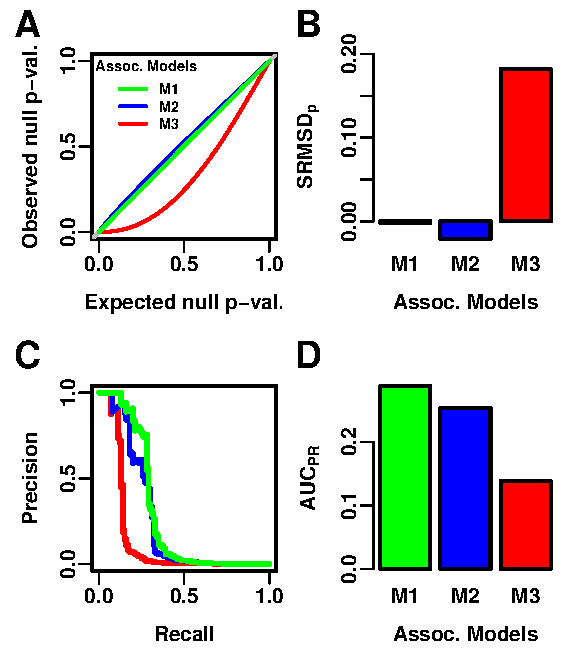
\includegraphics{sim-n1000-k10-f0.1-s0.5-g1/measures-illustration.pdf}
  \caption{
    {\bf Illustration of $\rmsd$ and $\auc$ evaluation measures.}
    Three archetypal models (M1, M2, M3) illustrate our two complementary measures.
    M1 is an ideal model that performs best overall, M2 overcorrects for population structure so it incurs a small performance penalty, and M3 does not correct for population structure so it performs most poorly.
    \textbf{A.}
    Probability-probability plot of the subset of p-values testing ``null'' (non-causal) loci.
    M1 has uniform null p-values as desired (overlaps $y=x$).
    M2/M3 have null p-values larger/smaller than expected.
    \textbf{B.}
    The $\rmsd$ (p-value Signed Root Mean Square Deviation) summarizes null p-value accuracy using a scaled Euclidean distance between the observed null p-values and their uniform expectation, with a negative sign if the median is larger than expected (closer to zero is better).
    \textbf{C.}
    Precision-Recall plot assesses causal locus classification performance across significance thresholds, without assuming that p-values are accurate (only locus ranks matter; higher is better).
    \textbf{D.}
    The $\auc$ (Precision-Recall Area Under the Curve) summarizes classification performance (higher is better).
  }
  \label{fig:measures_illustration}
\end{figure}

% PCA, LMM, PCs series
The overall goal is to characterize the performance of two association models: PCA and LMM.
Each of PCA and LMM was evaluated in each dataset while including a number $r$ of PCs as fixed covariates, in both cases varying $r$ between 0 and 90.
We determined which value of $r$ was optimal (in terms of $\rmsd$ and $\auc$ separately) for each of PCA and LMM separately, in each dataset, and lastly compared overall performance per dataset across the best PCA and LMM cases (with their optimal $r$ values).
Our overall statistical evaluation will be summarized first, followed by detailed evaluations in each datasets in the rest of the results.

We first describe the results for null p-value uniformity ($|\rmsd|$; \cref{tab:human_sum_pcs}).
Only here the sign of $\rmsd$ was ignored, so smaller is better and Wilcoxon paired 1-tailed tests were used to determine whether a suboptimal distribution was significantly different.
For PCA, the optimal number of PCs $r$ is typically large across all datasets (up to $r=90$, which was the largest value tested), but we found that much smaller ``min'' $r$ values often performed as well (numbers in parentheses in \cref{tab:human_sum_pcs} are the smallest $r$ whose $|\rmsd|$ distributions were not significantly different from the distribution of the $r$ with the smallest mean $|\rmsd|$).
However, even the min $r$ values for PCA tended to be large on the family simulations and the real datasets, compared to the admixture and tree simulations.
In most cases both the best $r$ and the min $r$ had a mean $|\rmsd| < 0.01$ (marked with asterisks), whose null p-value distributions effectively uniform.
Mean $|\rmsd| > 0.01$ cases for PCA were most common on the family simulation and real datasets.
In contrast, for LMM $r=0$ (no PCs) was always the optimal choice (always resulted in the minimum mean $|\rmsd|$), and in those cases we also always had mean $|\rmsd| < 0.01$.
Lastly, comparing the $|\rmsd|$ distributions between PCA and LMM, each with their best $r$, resulted in LMM besting often or in statistical ties, whereas PCA was best in the Human Origins simulations only.

\begin{table}[hb!]
  \centering
  %\scriptsize
  \caption{
    \textbf{Overview of PCA and LMM evaluation results}
  }
  \label{tab:human_sum_pcs}
  \csvreader[
  tabular = lc|ccc|ccc,
  separator = tab,
  table head = 
  % header row 1
  \toprule & Metric: & \multicolumn{3}{c|}{$|\rmsd|$} & \multicolumn{3}{c}{$\auc$} \\
  % header row 2
  \midrule & & \multicolumn{2}{c}{Best (min\textsuperscript{b}) PCs} & & \multicolumn{2}{c}{Best (min\textsuperscript{b}) PCs} & \\
  % header row 3
  Dataset & {Trait model\textsuperscript{a}} & PCA & LMM & {Best\textsuperscript{c}} & PCA & LMM & {Best\textsuperscript{c}} \\\midrule,
  late after last line = \\\bottomrule
  ]{../data/stats.txt}{}{\csvlinetotablerow}
  \begin{flushleft}
    \textsuperscript{a}FES: Fixed Effect Sizes, RC: Random Coefficients.\\
    \textsuperscript{b}Smallest $r$ (number of PCs) whose distribution ($|\rmsd|$ or $\auc$) was not significantly different (Wilcoxon paired 1-tailed $p > 0.01$) from the $r$ with best mean value (if any). \\
    \textsuperscript{c}Tie if distributions ($|\rmsd|$ or $\auc$) of best PCA and LMM version (previous two columns) did not differ significantly (Wilcoxon paired 1-tailed $p > 0.01$).
    Result was always the same whether ``best'' or ``min'' (in parenthesis) cases were compared, except in one case (in parenthesis).\\
    *$r$ for which mean $|\rmsd| < 0.01$ ($|\rmsd|$ columns only).
  \end{flushleft}
\end{table}

Next we turn to classification performance ($\auc$; \cref{tab:human_sum_pcs}).
For PCA, the best $r$ for $\auc$ was always smaller than the best $r$ for $|\rmsd|$, and also for the respective ``min'' $r$ comparisons (smallest $r$ which is not significantly different in $\auc$ distribution from the best $r$).
Thus, for PCA there is often a tradeoff between accurate p-values versus classification performance.
For LMM there is no such tradeoff, as $r=0$ (no PCs) resulted in $\auc$ distributions not significantly different from the best $r$ in all tests except one (in the 1000 Genomes simulation with the random coefficients trait model, the min $r$ was 1).
Lastly, LMM with its best $r$ always had significantly greater $\auc$ distributions than PCA with its best $r$.

\subsection{Evaluations in admixture simulations}

Now we look more closely at the results of every individual evaluation.
The $\rmsd$ and $\auc$ distributions for the first three admixture simulations and the \textit{fixed effect size} trait simulation are in \cref{fig:rmsd-auc-sim}.
We repeated the evaluation with traits simulated from the \textit{random coefficients} model as well, which gave qualitatively similar results (\cref{fig:rmsd-auc-sim-rc}).

The large admixture simulation differs from previous admixture evaluations in featuring a larger number of ancestral populations ($K=10$) and more differentiation ($\Fst = 0.1$ for the admixed individuals).
Admixture is structured over a one-dimensional geography \citep{ochoa_estimating_2021}.
The $\rmsd$ of PCA is largest when $r=0$ (no PCs) and decreases rapidly to zero at $r=3$, where it stays for up to $r=90$ (\cref{fig:rmsd-auc-sim}A).
Thus, PCA gives effectively accurate p-values for all $r \ge 3$, which is surprisingly smaller than the theoretical optimum for this simulation of $r = K - 1 = 9$.
In contrast, the $\rmsd$ distribution for LMM starts near zero for $r=0$, and as $r$ increases moves away from zero in the negative direction (null test statistics are deflated, so p-values become conservative).
The $\auc$ distribution of PCA is similarly worst at $r=0$, increases rapidly and peaks at $r = 3$, then decreases slowly for $r > 3$.
Similarly, the $\auc$ distribution for LMM starts near its maximum at $r=0$, and decreases overall for larger $r$.
Although the $\auc$ distributions for LMM and PCA overlap considerably at each $r$, LMM with $r=0$ has significantly greater $\auc$ values than PCA with $r=3$ (\cref{tab:human_sum_pcs}).
However, qualitatively PCA closely matches LMM in performance in this simulation.
Both LMM and PCA are robust to extreme values of $r$.

\begin{figure}[bp!]
  \centering
  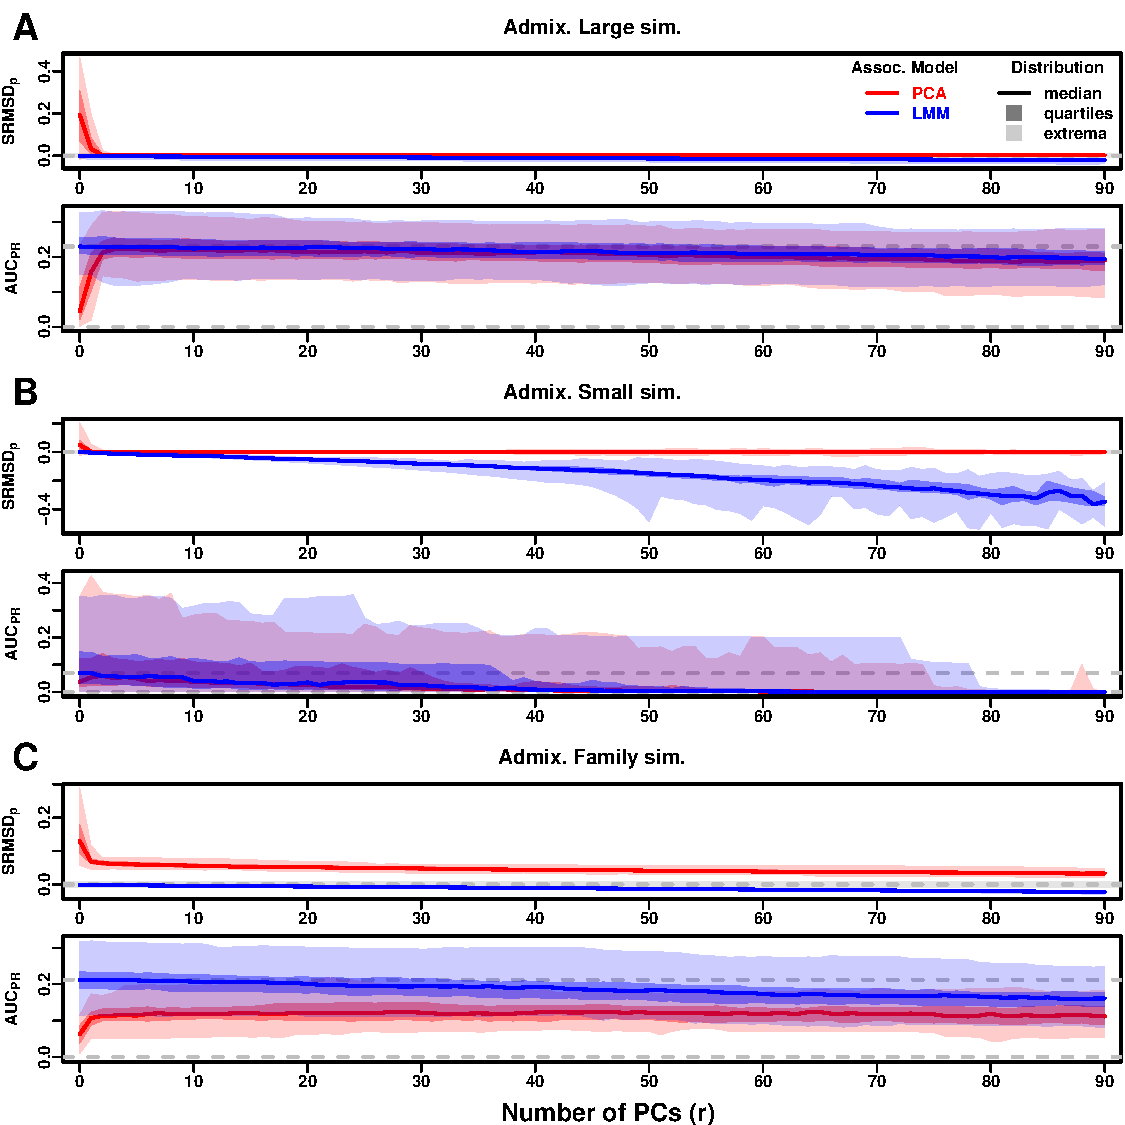
\includegraphics[width=\textwidth,height=\textheight,keepaspectratio]{fes/rmsd-auc-sim.pdf}
  \caption{
    {\small 
      {\bf Evaluations in admixture simulations.}
      Traits simulated from \textit{fixed effect sizes} model.
      PCA and LMM approaches are tested with varying number of PCs ($r \in \{0, ..., 90\}$ on x-axis), with the distributions (y-axis) of $\rmsd$ (top subpanel) and $\auc$ (bottom subpanel) for 50 replicates.
      Best performance is zero $\rmsd$ and large $\auc$.
      Zero values and maximum median $\auc$ values are marked with horizontal gray dashed lines, and the $|\rmsd| < 0.01$ band is marked with a light gray area.
      LMM always performs best when $r=0$, and PCA performs best when $r$ is between 1-4.
      \textbf{A.}
      The large simulation has $n = 1,000$ individuals.
      \textbf{B.}
      The small simulation has $n = 100$ individuals, shows overfitting for large $r$.
      \textbf{C.}
      The family simulation has $n = 1,000$ individuals from a family with admixed founders and large numbers of pairs of sibling, first/second cousins, etc, from a realistic random 20-generation pedigree.
      Here PCA performs poorly compared to LMM: $\rmsd > 0$ for all $r$, and a large gap in $\auc$.
    }
  }
  \label{fig:rmsd-auc-sim}
\end{figure}

The previous robustness to large $r$ led us to consider smaller sample sizes.
Our expectation is that a model with large numbers of parameters $r$ should overfit more as $r$ increases, and particularly as $r$ approaches the sample size $n$ (number of individuals).
Rather than increase $r$ beyond 90, which is not done in practice, we reduce individuals to $n = 100$, which is small for typical association studies but may occur in studies of rare diseases, pilot studies, or other constraints.
To compensate for the loss of power due to reducing $n$, we also reduce the number of causal loci from 100 before to $m_1 = 10$, (in all cases a fixed ratio of $n / m_1 = 10$) which increases the locus effect sizes.
As expected, we found a large decrease in performance for both PCA and LMM as $r$ increases, with optimal performance attained near $r=1$ for PCA and $r=0$ for LMM (\cref{fig:rmsd-auc-sim}B).
LMM attains much larger negative $\rmsd$ values than in our other evaluations.
While LMM with $r=0$ is significantly better than PCA ($r=1$ to 4) in both metrics (\cref{tab:human_sum_pcs}), qualitatively the difference is negligible.

The last of the first three simulations adds a 20-generation random family to our admixture simulation.
Previous work has reported, in limited settings, that PCA performs poorly in the presence of family structure, so it is important to establish the detailed behavior of PCA and LMM in this setting as $r$ is varied for both.
Since LMM is formulated in terms of kinship, it is expected to perform better here.
Only the last generation is studied for association, which contains numerous siblings, first cousins, etc.
The initial population structure due to admixture is preserved across the generations by strongly biasing mating pairs for proximity over the one-dimensional geography, which results in an indirect ancestry-biased assortative mating (see Methods).
Our evaluation reveals a sizable gap in both metrics between LMM and PCA across all values of $r$ (\cref{fig:rmsd-auc-sim}C).
LMM again performs best with $r=0$ and achieves mean $|\rmsd| < 0.01$.
However, PCA does not achieve zero $\rmsd$ at any $r$ value (all p-values are strongly anti-conservative), and the best mean $\auc$ value across $r$ for PCA is worse than the worst mean $\auc$ value for LMM.
Thus, LMM is conclusively superior to PCA, and the only calibrated model, when there is family structure.

\subsection{Evaluations in real human genotype datasets}

Next we repeat our evaluations with real human genotype data, which differs from our simulations in allele frequency distributions and more complex population structures with greater differentiation, numerous correlated subpopulations, and potential cryptic family relatedness.
We chose three datasets that span global human diversity and include both array and WGS genotyping platforms.
Loci in high linkage disequilibrium were removed to simplify our evaluation, and traits were simulated from these genotypes and each of the two trait models: fixed effect sizes (\cref{fig:rmsd-auc-real}) and random coefficients (\cref{fig:rmsd-auc-real-rc}).

Among the real datasets, Human Origins has the greatest number and diversity of subpopulations.
The $\rmsd$ and $\auc$ distributions in this dataset and the fixed effect sizes trait model (\cref{fig:rmsd-auc-real}A) most resemble those from the family simulation (\cref{fig:rmsd-auc-sim}C).
In particular, while LMM with $r=0$ again performed optimally (both metrics) and satisfies mean $|\rmsd| < 0.01$, PCA maintained mean $\rmsd > 0$ for all $r$ values and its $\auc$ values were all strictly smaller than even the worst $\auc$ values of LMM at any $r$.

\begin{figure}[bp!]
  \centering
  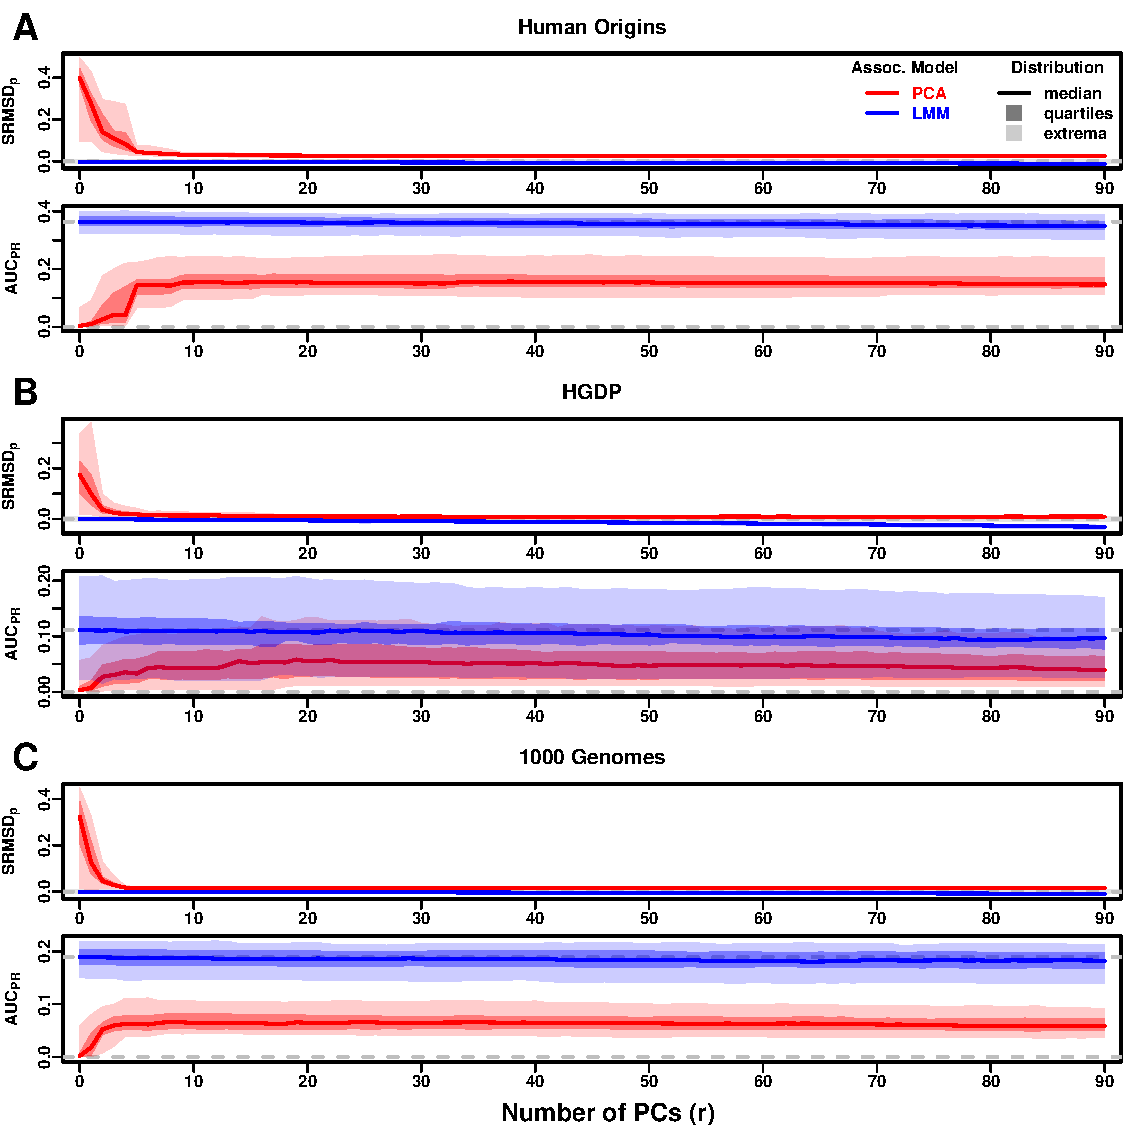
\includegraphics[width=\textwidth,height=\textheight,keepaspectratio]{fes/rmsd-auc-real.pdf}
  \caption{
    {\small 
      {\bf Evaluations in real human genotype datasets.}
      Traits simulated from \textit{fixed effect sizes} model.
      Same setup as \cref{fig:rmsd-auc-sim}, see that for details.
      These datasets strongly favor LMM with $r = 0$ PCs over PCA, resulting in curves that resemble the previous admixed family simulation, even though these datasets excluded known family members.
      \textbf{A.}
      The Human Origins dataset.
      \textbf{B.}
      The Human Genome Diversity Panel (HGDP) dataset.
      \textbf{C.}
      The 1000 Genomes Project dataset.
    }
  }
  \label{fig:rmsd-auc-real}
\end{figure}

The HGDP dataset has the fewest individuals among real datasets, but compared to Human Origins it contains many more loci and more low-frequency variants.
The $\rmsd$ and $\auc$ distributions (\cref{fig:rmsd-auc-real}B) are intermediate between the admixture and family simulations.
In particular, here both LMM ($r=0$) and PCA ($r \ge 31$) achieve mean $|\rmsd| < 0.01$, so null p-values will be accurate in both association models.
However, there is a sizable mean $\auc$ gap between LMM, which performed best across all values of $r$, and PCA.
Maximum $\auc$ values were lowest in HGDP compared to the two other human datasets.

1000 Genomes has the fewest subpopulations but a large number of individuals, and like HGDP is also WGS.
Thus, although this dataset is expected to have the simplest population structure among the real datasets, we find $\rmsd$ and $\auc$ distributions (\cref{fig:rmsd-auc-real}C) that again resemble those of our earlier family simulation, with mean $|\rmsd| < 0.01$ for LMM only and large $\auc$ gaps between LMM and PCA.

The previous results for the real datasets focused on traits drawn from the fixed effect sizes (FES) model.
In this case the results are qualitatively very different for traits drawn from the random coefficients (RC) model (\cref{fig:rmsd-auc-real-rc}).
The key difference is that $\auc$ gaps between LMM and PCA, which were very large in FES, are much smaller in RC.
Maximum $\auc$ were smaller in RC compared to FES in two of the three datasets.
$\rmsd$ distributions are practically the same in RC versus FES.
Nevertheless, our overall statistical evaluations declare LMM with $r=0$ superior to PCA in both RC and FES traits (\cref{tab:human_sum_pcs}).

\subsection{Evaluations in tree simulations fit to human data}

To better understand what features of the real datasets lead to the large differences in performance between LMM and PCA, we performed additional simulations.
In particular, human subpopulations are related roughly by a tree, which induces the strongest correlations (\cref{fig:kinship}), so we wanted to determine if this tree structure alone could recapitulate our previous results.
Thus, we fit trees to each human dataset and verified that the kinship matrices of the simulations were a rough match to those of the real datasets, as desired.
The second feature included in these simulations (absent in the admixture simulations) is a non-uniform ancestral allele frequency distribution, which recapitulated some of the skew for smaller minor allele frequencies of the real datasets (\cref{fig:kinship}C).

The $\rmsd$ and $\auc$ distributions for these tree simulations (\cref{fig:rmsd-auc-real-sim}) resembled our admixture simulation more than either the family simulation (\cref{fig:rmsd-auc-sim}) or real data results (\cref{fig:rmsd-auc-real}).
In all three of these simulations, both LMM with $r=0$ and PCA (various $r$) achieve mean $|\rmsd| < 0.01$, and in two out of the three cases both association models (with their best $r$) were not significantly different for $|\rmsd|$ (\cref{tab:human_sum_pcs}).
The $\auc$ distributions of both LMM and PCA track closely as $r$ is varied, although there is a small gap in performance that results in LMM ($r=0$) besting PCA in all three simulations.
The results are qualitatively similar for the random coefficients trait model (\cref{fig:rmsd-auc-real-sim-rc,tab:human_sum_pcs}).
Overall, the tree simulations do not recapitulate the large LMM advantage over PCA observed in the previous real human data results.

\begin{figure}[bp!]
  \centering
  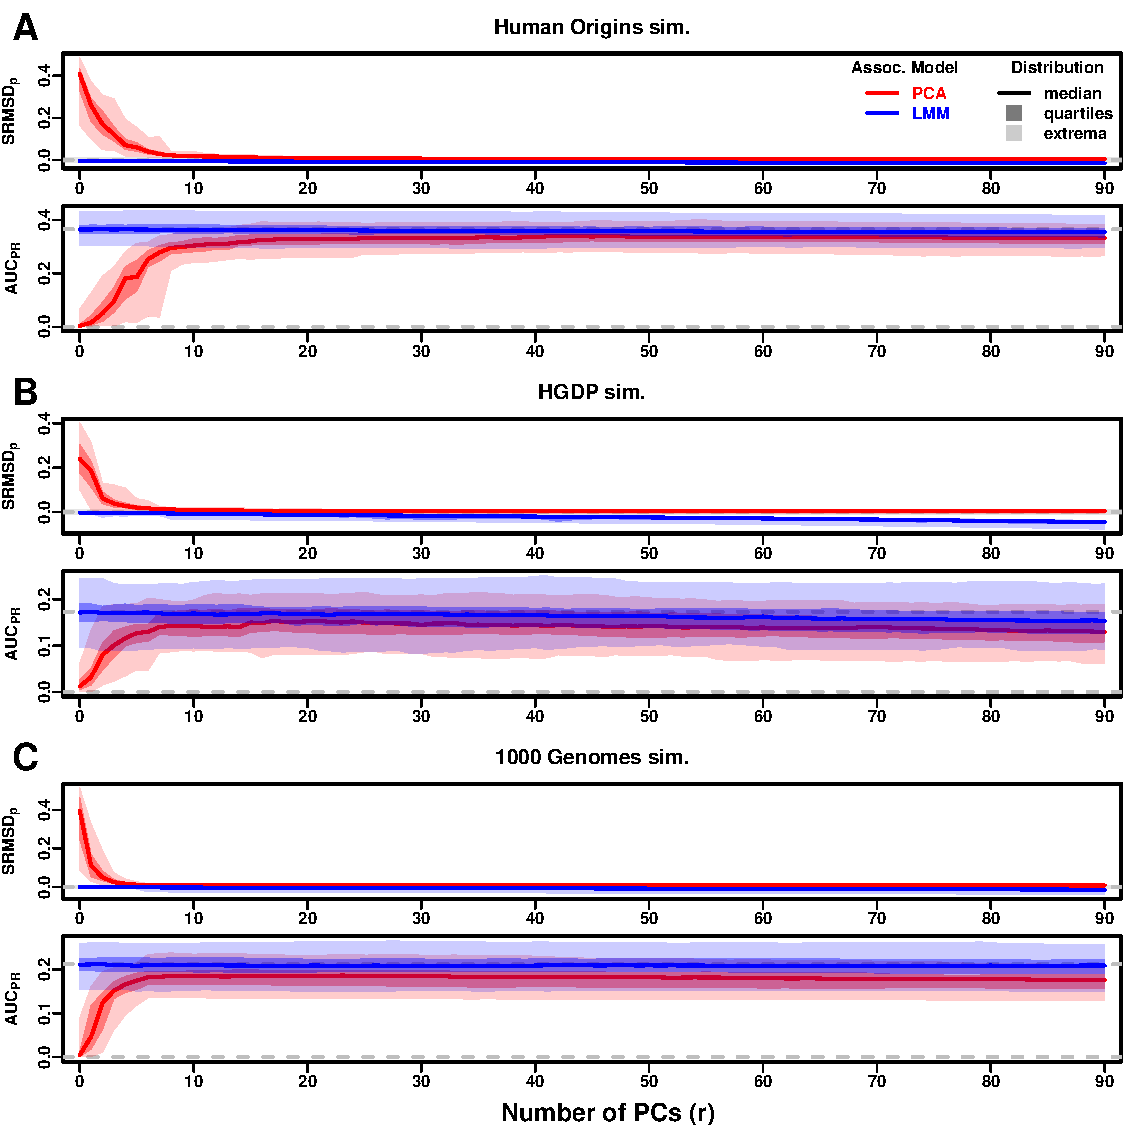
\includegraphics[width=\textwidth,height=\textheight,keepaspectratio]{fes/rmsd-auc-real-sim.pdf}
  \caption{
    {\small 
      {\bf Evaluations in tree simulations fit to human data.}
      Traits simulated from \textit{fixed effect sizes} model.
      Same setup as \cref{fig:rmsd-auc-sim}, see that for details.
      These tree simulations, which exclude within-subpopulation family structure by design, do not explain the large gaps in LMM-PCA performance observed in the real datasets.
      \textbf{A.}
      The Human Origins simulation.
      \textbf{B.}
      The Human Genome Diversity Panel (HGDP) simulation.
      \textbf{C.}
      The 1000 Genomes Project simulation.
    }
  }
  \label{fig:rmsd-auc-real-sim}
\end{figure}

\subsection{Estimated eigenvalues do not explain PCA performance}

A first-principles hypothesis for why PCA performs well in some datasets and not in others is their differences in dimensionality, since PCA assumes a low-dimensional genetic structure whereas LMM can model high-dimensional genetic structures.
We applied the Tracy-Widom statistical test \citep{patterson_population_2006} with $p < 0.01$ to determine the number of significant principal components in each dataset, which estimates the rank of the kinship matrix (i.e., its dimensionality).
These kinship ranks (\cref{fig:eigen}A) slightly underestimated the true dimensionality of our simulations (\cref{tab:human_sum}).
However, rank estimates agree that the admixed family simulation has the greatest rank, and that the real datasets have greater ranks than the admixture simulations and, to a lesser extent, their respective tree simulations.
However, these estimated ranks do not differentiate datasets where PCA performs well from those where performance was poor, particularly between the real and tree simulations, which span a similar range of ranks.
Moreover, the 1000 Genomes rank estimate is lower than 90, yet PCA performed poorly for all $r \ge 90$ numbers of PCs tested (\cref{fig:rmsd-auc-real}).
Performance might depend on the ratio of the matrix rank to its dimension (the number of individuals) or a more complicated formula, but the datasets tested do not differ greatly in dimensions (at most 3x, excluding the small simulation), while our analysis does not reveal an obvious line that separates these dataset by PCA performance.

We also compared eigenvalues across datasets, expressed as variance explained (each eigenvalue divided by the sum of eigenvalues) to facilitate comparisons across datasets.
The top eigenvalue explained a proportion of variance roughly proportional to \Fst (\cref{tab:human_sum}), but the rest of the top 10 eigenvalues show no large differences between datasets (\cref{fig:eigen}C), except the small admixture simulation had larger variances explained per eigenvalue (as expected since it has fewer eigenvalues).
We also visualized all eigenvalues (beyond the top 10), computing their cumulative variance explained distributions versus their eigenvalue rank fraction (normalized to account for sample size differences).
Each dataset has a different starting point, but all increase almost linearly from there until they reach 1, except for the family simulation, which has much greater variance explained by mid-rank eigenvalues (\cref{fig:eigen}B).
However, there are again no obvious clues separating datasets where PCA performed poorly (such as the real datasets) from those where it performed relatively well (such as the corresponding tree simulations).

\subsection{Local kinship explains PCA performance}

Local kinship, which is relatedness due to family structure ignoring population structure if present, is the presumed cause of the LMM to PCA gap observed in real datasets but not in their tree simulation counterparts.
Rather than measure its presence indirectly as increased dimensionality, as attempted in the previous section, here we measure it directly using the KING-robust estimator (\cref{fig:king}).
As expected, we observe more larger local kinship values in the real datasets and the family simulation compared to the admixture and tree the simulations.
However, this distribution in the real datasets depends on both sample size and number of subpopulations, as locally related pairs are most likely in the same subpopulation and conversely pairs between subpopulations tend to be negative for this estimator.
For these reasons, the only comparable curve to each real dataset is their corresponding tree simulation, which matches sample size and subpopulation structure.

\begin{figure}[bp!]
  \centering
  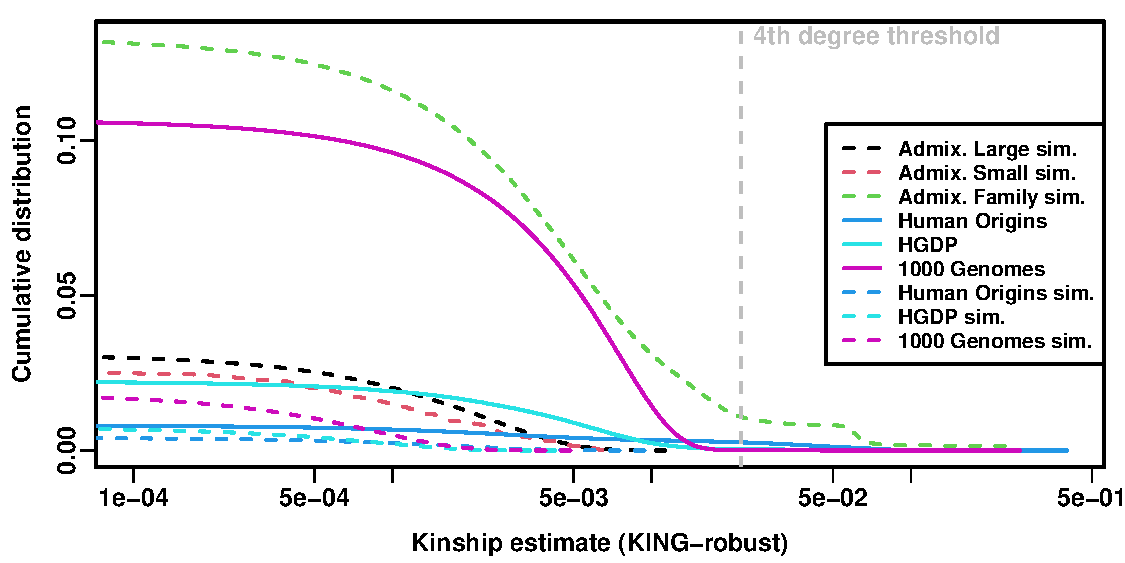
\includegraphics[width=\textwidth]{king_log-x.pdf}
  \caption{
    {\bf Local kinship estimate distribution.}
    Curves are the complementary cumulative distribution of all lower triangular kinship matrix values from the KING-robust estimator.
    Self kinship is excluded.
    Note log scale of x-axis; negative estimates are counted in cumulatives but not shown.
    The majority of values in all datasets are below the 4th degree relative threshold value.
    Real datasets have greater cumulative distributions at every kinship value compared to their respective tree simulations.
  }
  \label{fig:king}
\end{figure}

In all real datasets we identified highly related individual pairs, defined here as those with kinship values above the 4th degree relative threshold of 0.022 \citep{manichaikul_robust_2010, conomos_model-free_2016}.
However, these highly related pairs are vastly outnumbered by pairs who are less related but have greater than zero kinship, which may be inferred stringently as exceeding the maximum values in the corresponding tree simulations, $\approx 0.01$, or if we are more permissive in allowing some small fraction of false positives we might reasonably include values above 0.001 (\cref{fig:king}).

We tested whether removal of the small number of highly related individual pairs improves PCA performance or if the presence of larger numbers of more distantly related pairs are to blame for poor PCA performance.
After removing 4th degree relatives, which reduced sample sizes between 5\% and 10\% (\cref{tab:king_cutoff}). we find largely the same results as in the evaluation that included all individuals (\cref{fig:king_cutoff}).
For simplicity a single number of PCs was tested for each model, $r=0$ for LMM and $r=20$ for PCA, as these consistently performed well in our earlier evaluation with all individuals.
Similarly, only the fixed effect sizes trait was tested, as that previously showed a large gap in performance between association models, while the random coefficients trait had a much smaller gap.
LMM significantly outperformed PCA in all these cases (Wilcoxon paired 1-tailed $p < 0.01$).
Notably, PCA still had miscalibrated p-values in Human Origins and 1000 Genomes ($|\rmsd| > 0.01$).
Otherwise, $\auc$ and $\rmsd$ ranges were similar in this evaluation and the one with all individuals.
We therefore conclude that the small number of highly related individual pairs had a negligible effect in PCA performance, so it must be the larger number of more distantly related pairs that explain the poor PCA performance compared to LMM in the real datasets.

\begin{figure}[bp!]
  \centering
  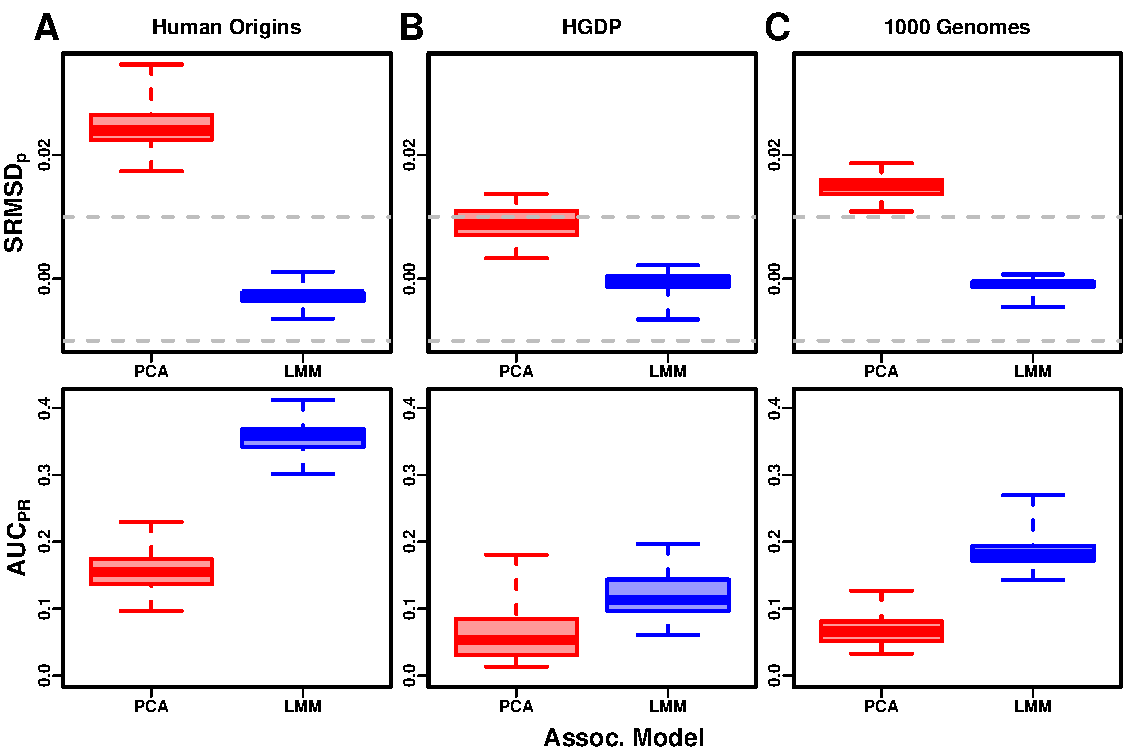
\includegraphics[width=\textwidth]{fes/rmsd-auc_king-cutoff-4.pdf}
  \caption{
    {\bf LMM and PCA performance in real datasets excluding 4th degree relatives.}
    LMM had $r=0$ PCs and PCA had $r=20$, and only fixed effect sizes trait model was tested.
    Each dataset is a column, rows are metrics.
    The $\rmsd$ cases (first row) have $|\rmsd| < 0.01$ band marked with dashed gray lines.
  }
  \label{fig:king_cutoff}
\end{figure}


\subsection{Comparison between $\rmsd$ and inflation factor}

Now that our main evaluation of the PCA and LMM models is concluded, we turn to a comparison of our new $\rmsd$ measure and the more common inflation factor.
Remarkably, there is a near one-to-one correspondence between $\lambda$ and our $\rmsd$ statistics (\cref{fig:rmsd_lambda}).
PCA tended to be inflated ($\lambda > 1$ and $\rmsd > 0$) whereas LMM tended to be deflated ($\lambda < 1$ and $\rmsd < 0$), otherwise the data for both models fall on the same contiguous curve.
One advantage of $\rmsd$ is that its range is limited, while $\lambda$ is unbounded and on a log scale.
We fit the following sigmoidal function to this data,
\begin{equation}
  \label{eq:rmsd_lambda_sigmoidal}
  \rmsd( \lambda ) = a \frac{ \lambda^b - 1 }{ \lambda^b + 1 },
\end{equation}
% inverse:
% lambda <- ( ( a + rmsd ) / ( a - rmsd ) )^(1/b)
which for all $a,b > 0$ satisfies $\rmsd( \lambda = 1 ) = 0$ and reflects $\log( \lambda )$ about zero ($\lambda = 1$) as desired, namely that
$$
\rmsd( \log( \lambda ) = -x ) = - \rmsd( \log( \lambda ) = x ).
$$
% \rmsd
% = a \frac{ e^{-bx} - 1 }{ e^{-bx} + 1 }
% = a \frac{ 1 - e^{bx} }{ 1 + e^{bx} }
We fit this model to the upper portion of the data only ($\lambda > 1$), since it was less noisy and of greater interest, and obtained the curve shown in \cref{fig:rmsd_lambda} with parameters $a = 0.566$ and $b = 0.616$.
% Using this model, we also produced a log-linear approximation based on its Taylor series with respect to $x = \log( \lambda )$ about $x=0$, resulting in
% \begin{equation}
%   \label{eq:rmsd_lambda_log_linear}
%   \rmsd( \lambda ) \approx \frac{a b}{2} \log( \lambda ).
% \end{equation}
% % inverse:
% % lambda <- exp( 2 * rmsd / ( a * b ) )
The value $\lambda = 1.05$, a threshold typically used to determine that there is no inflation \citep{price_new_2010}, corresponds to $\rmsd = 0.0085$ according to \cref{eq:rmsd_lambda_sigmoidal}.
Conversely, $\rmsd = 0.01$, serving as a simpler rule of thumb, corresponds to $\lambda = 1.06$.


\section{Discussion}

Our evaluations conclusively determined that LMM without PCs performs better than PCA (for any number of PCs) across all scenarios, including all real and simulated genotypes and two trait simulation models.
Although the addition of a few PCs does not greatly hurt the performance of LMM (except for small sample sizes), such additions never resulted in significantly improved perfomance either (barring one marginally significant case with a small effect size; \cref{tab:human_sum_pcs}), which aggrees with previous observations \citep{liu_controlling_2011} but contradicts others \citep{zhao_arabidopsis_2007, price_new_2010}.
Our findings make sense since the PCs are the eigenvectors of the kinship matrix used to model the random effects, so including both is redundant.

Previous work also suggested that PCA can outperform LMM when [TODO: harmonize with intro] there are loci under selection or otherwise highly differentiated \citep{price_new_2010, wu_comparison_2011, yang_advantages_2014}.
Our evaluations on real human data, which contain such loci in relevant proportions if they exist, do not replicate those observations.
However, the presence of cryptic relatedness on all of these datasets, which favors LMM, may obscure the effect.
Therefore, while we are not able to completely dismiss this potential PCA advantage, it probably plays a minor role in human studies.

Relative to LMM, the behavior of PCA fell into two extremes.
When PCA performed well, there was a (typically small) number of PCs that resulted in both near zero mean $\rmsd$ and mean $\auc$ near that of LMM without PCs.
Conversely, when PCA performed poorly, no choice for the number of PCs led to either acceptably low $\rmsd$ or acceptably large $\auc$.
PCA performed well in the admixture simulations (without families, both trait models), real human genotypes with random coefficients traits, and, to a lesser extent, the tree simulations (both trait models).
Conversely, PCA performed poorly in the admixed family simulation (both trait models) and the real human genotypes with fixed effect sizes traits.

PCA assumes that genetic structure is low-dimensional, whereas LMM can handle high-dimensional structures.
Thus, PCA performs well in the admixture simulation, which is explicitly low-dimensional (see Methods), as well as in tree simulations with few nodes with long branches, such as the trees we fit to the real human data, where a low-dimensional approximation suffices.
Conversely, PCA performs poorly under family structure because its kinship matrix is high-dimensional.
One theoretical inconvenience is that true kinship matrices are always full rank: for example, an unstructured population where all individuals are equally unrelated and outbred has a kinship matrix of $\mathbf{I}/2$, whose eigenvalues are all equal to $1/2$.
Nevertheless, population structure induces a more unbalanced eigenvalue distribution with a few very large eigenvalues (\cref{fig:eigen}), so we may define dimensionality in practice as the number of eigenvalues that exceed some small threshold.
However, evaluating the dimensionality of real datasets is challenging because estimated kinship (covariance) matrices result in noisy eigenvalues with skewed distributions.
We used the Tracy-Widom test to estimate dimensionality \citep{patterson_population_2006}, which gives estimates coherent with the simulation models, although it slightly underestimated their dimensionality (as expected since there may be low power to detect small eigenvalues, which were less important in our PCA evaluations as well).
Our local kinship analysis confirms that there is considerable cryptic relatedness in all real human datasets, which explains why LMM outperforms PCA there.
However, estimated eigenvalues and kinship matrix ranks by themselves do not fully explain when PCA will perform poorly.
Furthermore, our evaluations reveal that the trait model also determines the relative performance of PCA, so genotype-based eigenvalues alone cannot tell the full story.

The real human genotype results, which are the most relevant in practice, suggests that PCA is at best underpowered relative to LMMs, and at worst produces inflated statistics regardless of the numbers of PCs included.
Among our simulations, such poor performance with the same features was observed only in the admixed family simulation.
Direct local kinship estimation shows that there is considerable family relatedness in the real datasets absent in the corresponding tree simulations.
Admixture is not modeled in our tree simulations, but our other admixture simulations concluded that this feature by itself is not problematic for PCA.
Reanalysis of 1000 Genomes has identified hundreds of close relative pairs (a few as close as siblings or parent-children; \cite{gazal_high_2015, al-khudhair_inference_2015, fedorova_atlas_2016, schlauch_identification_2017}).
However, our evaluations showed that removal of these few highly related individuals does not improve PCA performance sufficiently, revealing the larger number of more distantly related pairs to be PCA's most serious obstacle.
Cryptic relatedness is expected to be prevalent in any large human dataset \citep{henn_cryptic_2012, shchur_number_2018}.
Furthermore, our fixed-effect-sizes trait model shows that the challenges of cryptic relatedness are exacerbated when rare variants have large coefficients.
Overall, the high-dimensionality induced by cryptic relatedness appears to be the key challenge for PCA-based association in modern datasets that is readily overcome by LMM.

Minor conclusions follow.
Our extensive evaluation also determined that PCA is robust to using a large number of PCs, often far beyond the optimal choice, which agrees with previous anecdotal observations \citep{price_principal_2006, kang_variance_2010}.
This is in contrast to using too few PCs, for which there is a large performance penalty.
The exception was the small simulation, where only a narrow range of PCs performed well.
Thus, when using PCA it is best to err on including too many PCs rather than too few.
Here LMM is simpler for users since there is no need to choose the number of PCs.
However, if an LMM has a large number of covariates relative to its sample size (in our case PCs, though we expect this to generalize) then p-values become too conservative/deflated, which is a weakness of LMM's use of the likelihood ratio test and its asymptotic $\chi^2$ distribution, which PCA overcomes with the more accurate t-test.
Post-hoc evaluations, or simulations such as ours, remain important in all cases to ensure that statistics are as expected.

Overall, our results lead us to always recommend the use of LMM over PCA for association studies.
Although PCA offer flexibility and speed compared to LMM, additional work is required to ensure that PCA is adequate, including identifying close relatives for exclusion (lowering sample size and resulting in wasted resources) followed by simulations or other evaluations of the output statistics, and even then there is no guarantee that PCA will perform as well as LMM, in terms of both type-I error control and power.
The presence of large numbers of distant relatives, expected on any real dataset, all but ensures that PCA will perform poorly in practice compared to LMM for association studies.
Our findings also suggest that other applications that employ PCA to control for population structure, such as polygenic models \citep{qian_fast_2020}, may enjoy gains in power by instead employing an LMM or some other high-dimensional population structure model capable of modeling both population structure and cryptic relatedness.
% This was one of the observations of a recent reevaluation of polygenic adaptation for height \citep{berg_reduced_2019}.
% TODO: add LASSO-LMM and such citations here?

% Since PCA matches the performance of LMM when there is no family structure, this argues against the simple characterization that either fixed or random effects are in principle superior models for association studies \citep{price_new_2010, sul_mixed_2013, price_response_2013, sul_population_2018}.

\section{Models and Methods}

\subsection{Models for genetic association studies}

Here we describe the complex trait and kinship models that motivates both the PCA and LMM models for genetic association studies.
The derivations of the PCA and LMM models from the general quantitative trait model are similar to previous presentations \citep{astle_population_2009, hoffman_correcting_2013}, but we emphasize the kinship model for random genotypes as being crucial for these connections, and make a clear distinction between the true kinship matrix and its most common estimator, which is biased \citep{ochoa_estimating_2021, ochoa_human}.

\subsubsection{The complex trait model and PCA approximation}

Let $\xij \in \{ 0, 1, 2 \}$ be the genotype at locus $i$ for individual $j$, which counts the number of reference alleles.
Suppose there are $n$ individuals and $m$ loci,
$\mathbf{X} = ( \xij )$ is their $m \times n$ genotype matrix, and
$\mathbf{y}$ is the length-$n$ (column) vector which represents trait value for each individual.
The additive linear model for a quantitative (continuous) trait is:
\begin{equation}
  \label{eq:trait}
  \mathbf{y}
  =
  \mathbf{1} \alpha + \mathbf{X}^\intercal \boldsymbol{\beta} + \boldsymbol{\epsilon}
  ,
\end{equation}
where
$\mathbf{1}$ is a length-$n$ vector of ones,
$\alpha$ is the scalar intercept coefficient,
$\boldsymbol{\beta}$ is the length-$m$ vector of locus coefficients,
$\boldsymbol{\epsilon}$ is a length-$n$ vector of residuals,
and the $\intercal$ superscript denotes matrix transposition.
The residuals are assumed to follow a normal distribution: $\epsilon_j \sim \text{Normal}(0, \sigma^2)$ independently for each individual $j$, for some residual variance parameter $\sigma^2$.
For simplicity, non-genetic covariates are not part of this model (or the PCA and LMM counterparts) but are trivial to include without changing any of our theoretical results.

In current datasets $m \gg n$, as there are millions of loci $m$ while most studies have many fewer than a million individuals $n$.
In this case the full model above cannot be fit, as there are more parameters ($m+1$, the length of $\boldsymbol{\beta}$ and $\alpha$) than datapoints ($n$, the length of $\mathbf{y}$) to fit.
The PCA model with $r$ PCs approximates the full model fit at a single locus $i$:
\begin{equation}
  \label{eq:pca_gwas}
  \mathbf{y}
  =
  \mathbf{1} \alpha + \mathbf{x}_i \beta_i + \mathbf{U}_r \boldsymbol{\gamma}_r + \boldsymbol{\epsilon}
  ,
\end{equation}
where $\mathbf{x}_i$ is the length-$n$ vector of genotypes at locus $i$ only,
$\beta_i$ is the coefficient for that locus,
$\mathbf{U}_r$ is an $n \times r$ matrix of PCs, and
$\boldsymbol{\gamma}_r$ is the length-$r$ vector of coefficients for the PCs.
This approximation follows from the singular value decomposition of the genotype matrix:
$\mathbf{X}^\intercal = \mathbf{U} \mathbf{D} \mathbf{V}^\intercal$,
where
$\mathbf{U}$ is an $n \times n$ matrix of the left singular vectors of $\mathbf{X}$,
$\mathbf{V}$ is an $m \times n$ matrix of its right singular vectors, and
$\mathbf{D}$ is an $n \times n$ diagonal matrix of its singular values.
Thus, in the full model we have
$\mathbf{X}^\intercal \boldsymbol{\beta} = \mathbf{U} \boldsymbol{\gamma}$,
where
$\boldsymbol{\gamma} = \mathbf{D} \mathbf{V}^\intercal \boldsymbol{\beta}$ is a length-$n$ vector.
The approximation consists solely of replacing $\mathbf{U} \boldsymbol{\gamma}$ (the full set of $n$ left singular vectors and their coefficients) with $\mathbf{U}_r \boldsymbol{\gamma}_r$ (the top $r$ singular vectors only, which is the best approximation of rank $r$).
Thus, the extra terms in the PCA model approximate the polygenic effect of the whole genome, and assumes that the locus $i$ being tested does not contribute greatly to this signal.

\textbf{Statistical significance.}
The null hypothesis is $\beta_j = 0$ (no association).
The null and alternative models are each fit (fitting the coefficients of the multiple regression, where $\beta_j$ is excluded under the null while it is fit under the alternative).
The resulting regression residuals are compared to each other using the t-test, yielding a two-sided p-value.
Note that many common PCA implementations trade this t-test for a less accurate $\chi^2$ test, which requires the overall degrees of freedom of the model to be much smaller than the number of individuals.

\subsubsection{Kinship model for genotypes}

To better motivate the most common PC estimator for genotype data, and to connect PCA to LMMs, we shall review the kinship model for genotypes.
Here genotypes are random variables with a mean and covariance structure given by
$$
\E[ \xij | T ]
=
2 \pit,
\quad\quad
\Cov( \xij, \xij[k] | T )
=
4 \pit ( 1 - \pit ) \kt,
$$
where $T$ denotes the ancestral population (on which random variables are conditioned upon), \pit is the ancestral allele frequency at locus $i$, and \kt is the kinship coefficient between individuals $j$ and $k$ \citep{malecot_mathematiques_1948, wright_genetical_1951, jacquard_structures_1970}.
Thus, the genotype matrix can be standardized using the true ancestral allele frequencies \pit, as
$$
\mathbf{X}_S
=
\left(
  \frac{
    \xij - 2 \pit
  }{
    \sqrt{4 \pit \left( 1 - \pit \right)}
  }
\right)
,
$$
which results in a kinship matrix estimator:
$$
\E
\left[
\frac{1}{m}
\mathbf{X}_S^\intercal
\mathbf{X}_S
\right]
=
\mathbf{\Phi}^T
,
$$
where $\mathbf{\Phi}^T = ( \kt )$ is the $n \times n$ kinship matrix (do not confuse the ancestral population superscript $T$ with the matrix transposition symbol $\intercal$).
Replacing the raw genotype matrix $\mathbf{X}$ with the standardized matrix $\mathbf{X}_S$ in the trait model of \cref{eq:trait} results in an equivalent model, as this covariate differs only by a linear transformation.
Thus, starting from standardized genotypes, the PCs of interest are equal in expectation to the top eigenvectors of the kinship matrix.

\subsubsection{Estimation of principal components from genotype data}

In practice, the matrix of principal components $\mathbf{U}_r$ in \cref{eq:pca_gwas} is calculated from an estimate of the earlier standardized genotype matrix $\mathbf{X}_S$, namely
\begin{equation*}
  \mathbf{\hat{X}}_S
  =
  \left(
    \frac{
      \xij - 2 \pith
    }{
      \sqrt{4 \pith \left( 1 - \pith \right)}
    }
  \right)
  ,
\end{equation*}
where the true ancestral allele frequency \pit is replaced by the estimate
$
\pith = \frac{1}{2n} \sum_{j = 1}^n \xij,
$
and results in the kinship estimate
\begin{equation}
  \label{eq:kinship_std}
  \mathbf{\hat{\Phi}}^T
  =
  \frac{1}{m}
  \mathbf{\hat{X}}_S^\intercal
  \mathbf{\hat{X}}_S
  .
\end{equation}
This kinship estimate and minor variants are also employed in LMMs \citep{yang_gcta:_2011}.
This estimator of the kinship matrix is biased, and this bias is different for every individual pair \citep{ochoa_estimating_2021, ochoa_human}.
However, in regression-based genetic association models such as PCA and LMM, the existing approach performs as well as when the above estimate is replaced by the true kinship matrix (data not shown).
%The explanation, briefly, is that the biased expectation of the above estimator differs from the true kinship matrix by a rank-1 update, which is exactly compensated for by the intercept term $\mathbf{1} \alpha$ in \cref{eq:pca_gwas}.
%[TODO: cite BIAS GWAS]

\subsubsection{Connection between PCs and ancestry proportions}

Here we show that genetic association using ancestry proportions as covariates is equivalent in expectation to using PCs under the assumptions of the admixture model (\textit{i.e.}, there are no other forms of relatedness), which has been demonstrated empirically before \citep{alexander_fast_2009, zhou_strong_2016}.
We shall assume the following individual-specific admixture model commonly assumed when inferring ancestry proportions \citep{pritchard_inference_2000, falush_inference_2003, alexander_fast_2009, gopalan_scaling_2016, cabreros_likelihood-free_2019}.
There are $K$ subpopulations and every individual $j$ draws a proportion $q_{ju}$ of its alleles from subpopulation $S_u$, so ancestry proportions are non-negative and sum to one for every individual $j$.
Each subpopulation $S_u$ has an allele frequency $p_i^{S_u}$ at locus $i$, and thus the individual-specific allele frequency $\pi_{ij}$ of individual $j$ at locus $i$ is the mean subpopulation allele frequencies weighted by the ancestry proportions:
\begin{equation}
  \label{eq:admix}
  \pi_{ij} = \sum_{u=1}^K q_{ju} p_i^{S_u}.
\end{equation}
Genotypes are the sum of alleles drawn independently from this frequency, or $\xij | \pi_{ij} \sim \text{Binomial}(2, \pi_{ij})$.
Thus, the rowspace of the genotype matrix equals in expectation that of the individual-specific allele frequency matrix, which by \cref{eq:admix} is the same as the rowspace of the $n \times K$ admixture proportions matrix $\mathbf{Q} = (q_{ju})$.
Therefore, the top $K$ principal components suffice to fully model the rowspace of the genotypes, which only have dimension $K$.
Moreover, since an intercept term is always included in association models ($\mathbf{1} \alpha$ in \cref{eq:pca_gwas}), and the sum of rows of $\mathbf{Q}$ sums to one, then the rowspace of the combined model has dimension $K$ as well, so only $K-1$ PCs (plus intercept) are needed to span the rowspace of this admixture model.

\subsubsection{Linear mixed-effects model}

The LMM is another approximation to the complex trait model in \cref{eq:trait}.
Most LMM implementations support fixed covariates (how we combine LMM with PCs), but for simplicity we exclude them in this presentation of the classical LMM, which is
\begin{equation}
  \label{eq:lmm_gwas}
  \mathbf{y}
  =
  \mathbf{1} \alpha + \mathbf{x}_i \beta_i + \mathbf{s} + \boldsymbol{\epsilon}
  ,
\end{equation}
which is like the PCA model in \cref{eq:pca_gwas} except that the PC terms $\mathbf{U}_r \boldsymbol{\gamma}_r$ are replaced by the random effect $\mathbf{s}$, which is a length-$n$ vector drawn from \citep{sul_population_2018}
$$
\mathbf{s} \sim \text{Normal} \left( \mathbf{0}, \sigma^2_s \mathbf{\Phi}^T \right),
$$
where $\mathbf{\Phi}^T$ is the kinship matrix and $\sigma^2_s$ is a trait-specific variance scaling factor.
This model is derived from treating the standardized genotype matrix $\mathbf{X}_S$ as random rather than fixed, so that the standardized genetic effect
$\mathbf{X}_S^\intercal \boldsymbol{\beta}_S$
in \cref{eq:trait} has mean zero and a covariance matrix of
$$
\Cov \left( \mathbf{X}_S^\intercal \boldsymbol{\beta}_S \right)
=
|| \boldsymbol{\beta}_S ||^2 \mathbf{\Phi}^T
.
$$
The above random effect $\mathbf{s}$ satisfies those equations, where the variance scale equals $\sigma^2_s = || \boldsymbol{\beta}_S ||^2$.
Thus, PCA is the fixed model equivalent of LMM under the additional approximation that only the top $r$ eigenvectors are used, whereas LMM uses all eigenvectors.
A more explicit comparison follows in the next subsection.

Another advantage of LMM over PCA is that it has fewer parameters to fit: ignoring the shared terms in \cref{eq:pca_gwas} and \cref{eq:lmm_gwas}, PCA has $r$ parameters to fit (each PC coefficient in the $\boldsymbol{\gamma}$ vector), whereas LMMs only fit one additional parameter, namely $\sigma^2_s$.
Therefore, PCA is expected to overfit more substantially than LMM---and thus lose power---when $r$ is very large, and especially when the sample size (the number of individuals $n$) is very small.
Statistical significance in LMMs most often employs a likelihood ratio test, whose test statistic has a asymptotic $\chi^2$ distribution under the null hypothesis.

\subsubsection{Connection between LMM and PCA}

The LMM of \cref{eq:lmm_gwas} can be written to resemble more greatly the PCA model of \cref{eq:pca_gwas} \citep{astle_population_2009, hoffman_correcting_2013}:
\begin{equation}
  \label{eq:lmm_gwas_evd}
  \mathbf{y}
  =
  \mathbf{1} \alpha + \mathbf{x}_i \beta_i + \mathbf{U} \boldsymbol{\gamma}_\text{LMM} + \boldsymbol{\epsilon}
  , \quad\quad
  \boldsymbol{\gamma}_\text{LMM} = \sigma_s \boldsymbol{\Lambda}^{1/2} \mathbf{r}
  ,
\end{equation}
where $\mathbf{U}$ is the complete matrix of PCs (all $n$ of them), $\boldsymbol{\Lambda}$ is the diagonal matrix of eigenvalues of the kinship matrix such that its eigendecomposition is $\mathbf{\Phi}^T = \mathbf{U} \boldsymbol{\Lambda} \mathbf{U}^\intercal$, and $\mathbf{r} \sim \text{Normal}(\mathbf{0},\mathbf{I})$ is a standard normal random effect.
The connection follows since $\mathbf{s} = \sigma_s \mathbf{U} \boldsymbol{\Lambda}^{1/2} \mathbf{r}$ satisfies
$$
\mathbf{s} \sim \text{Normal} \left( \mathbf{0}, \left( \sigma_s \mathbf{U} \boldsymbol{\Lambda}^{1/2} \right) \left( \sigma_s \mathbf{U} \boldsymbol{\Lambda}^{1/2} \right)^\intercal \right)
= \text{Normal}( \mathbf{0}, \sigma_s^2 \mathbf{\Phi}^T ),
$$
which itself follows from the affine transformation property of multivariate normal distributions.
$\mathbf{U}$ also equals in the limit the right singular vectors of the standardized genotype matrix $\mathbf{X}_S = \mathbf{V}_S \mathbf{D}_S \mathbf{U}_S^\intercal$, which is how we originally motivated PCA, since
$$
\frac{1}{m} \mathbf{X}_S^\intercal \mathbf{X}_S
%= \frac{1}{m} \mathbf{U}_S \mathbf{D}_S \mathbf{V}_S^\intercal \mathbf{V}_S \mathbf{D}_S \mathbf{U}_S^\intercal
= \mathbf{U}_S \mathbf{\Lambda}_S \mathbf{U}_S^\intercal
\toas
\mathbf{U} \mathbf{\Lambda} \mathbf{U}^\intercal
=
\mathbf{\Phi}^T
$$
since $\mathbf{V}_S$ is orthonormal, and where $\mathbf{\Lambda}_S = \frac{1}{m} \mathbf{D}_S^2$.

Therefore, when the true kinship matrix is low-dimensional, the LMM fits the same low-dimensional space as PCA would with an appropriate number of PCs, except that the coefficients $\boldsymbol{\gamma}_\text{LMM}$ are constrained by the likelihood model, whereas the analogous PCA coefficients $\boldsymbol{\gamma}_r$ are unconstrained parameters.
On the other hand, when the kinship matrix is high-dimensional then the LMM can fit this space better than a corresponding PCA model with a small number of PCs, while PCA with a larger number of PCs will instead overfit the data.

\subsection{Simulations}

Let $\f{A}{B}$ denote the inbreeding coefficient of a subpopulation $A$ from another subpopulation $B$ that is ancestral to $A$.
Often we use $\ft[A]$ where $T$ is an overall ancestral population (ancestral to every subpopulation and/or individual under consideration, such as the most recent common ancestor population).
[TODO: introduce more notation here, or do it all earlier?]

\subsubsection{Genotype simulation from the admixture model}

We consider three admixture simulation scenarios, refered to as Large, Small, and Family.
The basic admixture model is as described previously \citep{ochoa_fst1, ochoa_estimating_2021}.

Large and Family have $n = 1,000$ individuals, while Small has $n = 100$.
The number of loci in all cases is $m = 100,000$.
Individuals are admixed from $K = 10$ intermediate subpopulations, or ancestries.
Each subpopulation $S_u$ ($u \in \{ 1, ..., K \}$) lies at coordinate $u$ and has an inbreeding coefficient $\ft[S_u] = u \tau$ for some $\tau$.
Ancestry proportions $q_{ju}$ for individual $j$ and subpopulation $S_u$ arise from a random walk model on the given 1-dimensional geography with spread $\sigma$, and the free parameters $\tau$ and $\sigma$ are fit to result in $\Fst = 0.1$ and mean kinship $\bar{\theta}^T = 0.5 \Fst$ for the admixed individuals, as before \citep{ochoa_estimating_2021}.

Random allele frequencies and genotypes are drawn from this hierarchical model:
\begin{align*}
  \pit
  &\sim
    \text{Uniform}( 0.01, 0.5 )
    , \\
  p_i^{S_u} | \pit
  &\sim
    \text{Beta} \left(
    \pit \left( \frac{1}{ \ft[S_u] } - 1 \right),
    \left( 1 - \pit \right) \left( \frac{1}{ \ft[S_u] } - 1 \right)
    \right)
    , \\
  \pi_{ij}
  &=
    \sum_{u = 1}^K q_{ju} p_i^{S_u}
    , \\
  \xij | \pi_{ij}
  &\sim
    \text{Binomial}(2, \pi_{ij})
    .
\end{align*}
Briefly, allele frequencies \pit for the ancestral population $T$ are drawn independently per locus $i$.
Subpopulation allele frequencies $p_i^{S_u}$ are drawn independently for each intermediate subpopulation $S_u$ from the Balding-Nichols distribution with mean \pit and variance $\pit \left( 1 - \pit \right) \ft[S_u]$ \citep{balding_method_1995}.
Lastly, the individual-specific allele frequencies $\pi_{ij}$ and genotypes \xij are as described earlier (\cref{eq:admix}).
Fixed loci ($i$ where $\xij = 0$ for all $j$, or $\xij = 2$ for all $j$) are drawn again from the model, starting from \pit, iterating until no loci are fixed.
Each replicate draws a new genotype matrix starting from new ancestral allele frequencies.

\subsubsection{Genotype simulation from random admixed families}

We simulated a pedigree with admixed founders that features:
(1) strict avoidance of close relatives when pairing individuals;
(2) favoring of close pairs in their 1-dimensional geography, which helps preserve the population structure by preferentially pairing individuals with similar admixture proportions (a form of assortative mating); and
(3) many generations, resulting in a distribution of close and distant relatives.

The 20 generations are drawn iteratively.
Generation 1 has individuals with genotypes drawn from the large admixture simulation described earlier.
These individuals are ordered by the 1-dimensional geography of the admixture scenario.
The local kinship matrix measures the pedigree relatedness; in the first generation, everybody is locally unrelated and outbred.
Individuals are randomly assigned to male or female with equal probability.

The children of the previous generation serve as the parents in the next generation, paired iteratively as follows.
From the pool of available males, one is picked randomly and is paired with the nearest female that is not a second cousin or closer relative (local kinship must be $< 1/4^3$); males that are not pairable are removed from the pool of available males.
Pairing stops when there are no more available males or females.

Next, a random number of children per pair is constructed to yield a desired population size $n$ and a minimum family size of $n_m=1$, as follows.
Let $n_f$ the be number of families (paired parents) in the current generation, then the number of additional children (beyond the minimum) is drawn from a Poisson distribution with parameter $n/n_f - n_m$.
Although the mean population size is $n$ as desired, the random sample may deviate from this target size.
Let $\delta$ be the difference between desired and current population sizes.
If $\delta > 0$, then $\delta$ random families are incremented by 1.
If $\delta < 0$, then $|\delta|$ random families with at least $n_m+1$ children are decremented by 1.
If $|\delta|$ exceeds the number of families, all families are incremented or decremented as needed and the process is iterated.
Children are assigned sex randomly, and are reordered by the average coordinate of their parents, preserving the original order when there are ties.

A new random pedigree was drawn for each replicate, as well as new genotypes for the founders drawn anew from the admixture model.
Genotypes are drawn across the pedigree, children drawing alleles from their parents independently per locus.

\subsubsection{Genotype simulation from a tree model}

A variant of the earlier admixture simulation model consists of drawing subpopulations allele frequencies from a hierarchical model, parametrized by a tree.
The ancestral population $T$ is at the root of the tree, and each node in the tree is a subpopulation $S_w$, where the nodes are indexed ($w$) arbitrarily.
Each edge between $S_w$ and its parent population $P_w$ has an inbreeding coefficient \f{P_w}{S_w}.
Allele frequencies are drawn from the root to the tips of the tree iteratively, as a hierarchical or graphical model, since this tree is a directed acyclic graph.
For the root $T$, allele frequencies \pit are drawn from a given distribution constructed to mimic each given real dataset (see below).
Given the allele frequencies $p_i^{P_w}$ of the parent population $P_w$, the child population $S_w$'s allele frequencies are drawn from the following Balding-Nichols distribution:
$$
p_i^{S_w} | p_i^{P_w}
\sim
\text{Beta} \left(
  p_i^{P_w} \left( \frac{1}{ \f{P_w}{S_w} } - 1 \right),
  \left( 1 - p_i^{P_w} \right) \left( \frac{1}{ \f{P_w}{S_w} } - 1 \right)
\right)
.
$$
Finally, individuals $j$ in the tip subpopulation $S_w$ have genotypes drawn independently from its allele frequency:
$$
\xij | p_i^{S_w}
\sim
\text{Binomial}\left( 2, p_i^{S_w} \right)
.
$$

To match the real datasets, which had loci with $\text{MAF} = \min \left\{ \pith, 1 - \pith \right\} < 0.01$ removed, our simulations had loci equivalently ascertained:
loci with $\text{MAF} < 0.01$ are drawn again from the model, starting from drawing a new \pit from the input distribution, iterating until no such loci remain.

\subsubsection{Fitting tree to data}

We developed new methods to fit trees to real data based on estimating kinship using \texttt{popkin}.
The general approach is divided into these parts:
deriving a simple additive estimation model,
estimating population-averaged coancestry values,
estimating tree topology, and
estimating inbreeding edge values for a given tree topology.

\textbf{Estimation model.}
A tree with given inbreeding edges gives rise to a specific coancestry matrix, which we calculate recursively here.
Suppose as before that every node in the tree, including root and tip nodes, are indexed as $S_w$.
Coancestry values $\vartheta_{uv}^T$ for a pair of subpopulations $S_u$ and $S_v$ are total inbreeding values of subpopulations in the tree.
In particular, the self-coancestry of $S_u$ equals its total inbreeding coefficient ($\vartheta_{uu}^T = \ft[S_u]$), and the coancestry of subpopulations $S_u$ and $S_v$ equals the total inbreeding of the most recent common ancestor (MRCA) population of those subpopulations:
$$
\vartheta_{uv}^T
=
\ft[ S_w ]
,
\quad\quad
S_w = \text{MRCA}( S_u, S_v )
.
$$
Since the above $S_w$ is always some node in the tree, we obtain the coancestry matrix by calculating the total inbreeding values of every $S_w$.

We will calculate total coancestries (from the ancestral population $T$, namely $\ft[S_w]$) for every node $S_w$ recursively through the tree branches from the root, as follows.
Recall the value of the edge to $S_w$ from its parent $P_w$ is $\f{P_w}{S_w}$, which is given.
Nodes whose parent is $P_w = T$ are already of the desired form.
If \ft[P_w] has been calculated, then \ft[S_w] is given by
$$
\ft[S_w] = \ft[P_w] + \f{P_w}{S_w} \left( 1 - \ft[P_w] \right),
$$
which is a special case of a previous calculation for three nested subpopulations \citep{ochoa_fst1}.
Note that the previous calculation is nearly additive, but instead of adding $\f{P_w}{S_w}$ to $\ft[P_w]$ we have to shrink $\f{P_w}{S_w}$ first by a factor of $\left( 1 - \ft[P_w] \right)$.
Define the additive contribution of the edge to $S_w$ as
$$
\delta_w = \ft[S_w] - \ft[P_w] = \f{P_w}{S_w} \left( 1 - \ft[P_w] \right).
$$
These $\delta_w \ge 0$ because $0 \le \f{P_w}{S_w}, \ft[P_w] \le 1$ for every $w$.
Importantly, the inbreeding edge values can be recovered from these additive edges recursively from the root, since nodes $S_w$ connected to the root satisfy
$\f{P_w}{S_w} = \ft[S_w] = \delta_w$,
and given $\ft[P_w]$ we can calculate $\f{P_w}{S_w}$ and $\ft[S_w]$ using
\begin{equation*}
  \f{P_w}{S_w}
  =
  \frac{ \delta_w }{ 1 - \ft[P_w] },
  \quad
  \ft[S_w]
  =
  \ft[P_w] + \delta_w
  .
\end{equation*}

The coancestry values are simplified as a sum of additive contributions $\delta_w$ for the nodes that are ancestors of the given pair of subpopulations,
\begin{equation}
  \label{eq:coanc_tree_additive}
  \vartheta_{uv}^T
  =
  \sum_w \delta_w I_w(u,v)
  ,
\end{equation}
where the sum goes over all nodes $S_w$ in the tree, and $I_w(u,v)$ is an indicator function equal to 1 if $S_w$ is an ancestor to both $S_u$ and $S_v$, and 0 otherwise.
Note that $I_w(u,v)$ are given by the tree topology, while $\delta_w$ reflect the edge values.
Therefore, given a topology, $\delta_w$ can be estimated by non-negative linear regression (see below), where $I_w(u,v)$ define the design matrix.

\textbf{Estimating population-averaged coancestry.}
Kinship (\ktHat) is estimated using \texttt{popkin} \citep{ochoa_estimating_2021}.
Coancestry ($\hat{\theta}_{jk}^T$) is estimated from kinship by replacing self-kinship with inbreeding (\ftHat) along the diagonal:
\begin{equation}
  \label{eq:kinship_to_coanc}
  \hat{\theta}_{jk}^T
  =
  \begin{cases}
    \ktHat & \text{if} \quad k \ne j, \\
    \ftHat = 2 \ktHat[j] - 1 & \text{if} \quad k = j.
  \end{cases}
\end{equation}
Lastly, coancestry values $\hat{\vartheta}_{uv}^T$ between subpopulations $S_u$ and $S_v$ are averages of the individual coancestry values across subpopulations, or within the subpopulation when $u=v$:
$$
\hat{\vartheta}_{uv}^T
=
\frac{1}{|S_u||S_v|} \sum_{j \in S_u} \sum_{k \in S_v} \hat{\theta}_{jk}^T
.
$$

\textbf{Estimating tree topology.}
Our topology estimation approach is remarkably simple, stemming from the monotonic relationship between node depth and coancestry from \cref{eq:coanc_tree_additive}.
Topology is estimated with hierarchical clustering using the weighted pair group method with arithmetic mean (WPGMA) algorithm \citep{sokal_statistical_1958}.
The distance function between subpopulations is
$$
d( S_u, S_v ) = \hat{\vartheta}_\text{max}^T - \hat{\vartheta}_{uv}^T,
$$
where $\hat{\vartheta}_\text{max}^T$ is the maximum $\hat{\vartheta}_{uv}^T$.
This algorithm recovers the true tree topology when the true coancestry values are provided, and performs well when $\hat{\vartheta}_{uv}^T$ are noisy estimates from genotypes.
However, edge lengths as estimated by hierarchical clustering are incorrect and ignored, fit in the next step.

\textbf{Estimating tree edge lengths.}
Additive edge lengths $\delta_w$ are estimated from \cref{eq:coanc_tree_additive} from the estimated subpopulation coancestry matrix $\hat{\vartheta}_{uv}^T$, using non-negative least squares linear regression \citep{lawson_solving_1974}, which minimizes the sum of squared residuals to the data while ensuring that every estimated coefficient $\delta_w$ is non-negative.
The desired inbreeding edge values $\f{P_w}{S_w}$ are then estimated from these $\delta_w$ using the recursive algorithm described earlier.
To account for small biases in coancestry estimation, an intercept term $\delta_0$ is fit (with $I_0(u,v) = 1$ for all $u,v$), and when converting $\delta_w$ to $\f{P_w}{S_w}$ values this is treated as an additional edge from the root of the input topology and the new root.
However, $\delta_0$ is ignored when drawing allele frequencies from the estimated tree.

\subsubsection{Fitting ancestral allele frequency distribution to data}

We calculated the allele frequency distribution \pith of each real dataset.
However, differentiation increases the variance of \pith relative to the true ancestral allele frequency \pit \citep{ochoa_estimating_2021}.
Here we present a new procedure for constructing an ``undifferentiated'' distribution of ancestral allele frequencies based on the input data \pith but which has the lower variance of the true \pit distribution.

\textbf{Model.}
Suppose the \pit distribution over all loci $i$ satisfies $\E \left[ \pit \right] = \frac{1}{2}$ (it is symmetric about 0.5) and $\Var \left( \pit \right) = V^T$.
The sample allele frequency \pith was previously found to have a conditional mean and variance (treating \pit as fixed) of
$$
\E \left[ \pith \middle| \pit \right]
=
\pit
, \quad\quad
\Var \left( \pith \middle| \pit \right)
=
\pit \left( 1 - \pit \right) \bar{\varphi}^T
,
$$
where $\bar{\varphi}^T = \frac{1}{n^2} \sum_{j=1}^n \sum_{k=1}^n \kt$ is the mean kinship over all individual \citep{ochoa_estimating_2021}.
The desired moments of the total (unconditional) distribution of \pith are given by the laws of total expectation and variance:
\begin{align*}
  \E \left[ \pith \right]
  &=
    \E \left[ \E \left[ \pith \middle| \pit \right] \right]
    =
    \E \left[ \pit \right]
    =
    \frac{1}{2}
    , \\
  W^T
  =
  \Var \left( \pith \right)
  &=
    \E \left[ \Var \left( \pith \middle| \pit \right) \right ]
    + \Var \left( \E \left[ \pith \middle| \pit \right] \right)
  \\
  &=
    \E \left[ \pit \left( 1 - \pit \right) \bar{\varphi}^T \right]
    + \Var \left( \pit \right)
    % \\
    % &=
    % \left( \E \left[ \pit \left( 1 - \pit \right) \right] \right) \bar{\varphi}^T
    % + \Var \left( \pit \right)
    % \\
    % &=
    % \left( \E \left[ \pit \right] - \E \left[ \left( \pit \right)^2 \right] \right) \bar{\varphi}^T
    % + \Var \left( \pit \right)
    % \\
    % &=
    % \left( \E \left[ \pit \right] - \left( \Var \left( \pit \right) + \left( \E \left[ \pit \right] \right)^2 \right) \right) \bar{\varphi}^T
    % + \Var \left( \pit \right)
  \\
  &=
    \bar{\varphi}^T \E \left[ \pit \right] \left( 1 - \E \left[ \pit \right] \right)
    + \left( 1 - \bar{\varphi}^T \right) \Var \left( \pit \right)
  \\
  &=
    \bar{\varphi}^T \frac{1}{4}
    + \left( 1 - \bar{\varphi}^T \right) V^T
    .
\end{align*}
Since $V^T \le \frac{1}{4}$ and $\bar{\varphi}^T \ge 0$, the variance of \pith is greater: $W^T \ge V^T$.
Thus, given $W^T$ and $\bar{\varphi}^T$, the goal is to construct a new distribution with the original, lower variance of
\begin{equation}
  \label{eq:var_undiff}
  V^T
  =
  \frac{ W^T - \frac{1}{4} \bar{\varphi}^T }{ 1 - \bar{\varphi}^T }
  .
\end{equation}

\textbf{Estimation of ancestral variance.}
Given empirical sample allele frequencies \pith, we use an unbiased sample estimator for $W^T$ that assumes a known expectation of one half, which is appropriate treating the choice of reference allele as random:
$$
\hat{W}^T
=
\frac{1}{m} \sum_{i=1}^m \left( \pith - \frac{1}{2} \right)^2
.
$$
The mean kinship $\bar{\varphi}^T$ is calculated from the tree simulation parameters: the subpopulation coancestry matrix calculated using \cref{eq:coanc_tree_additive}, expanded so rows and columns corresponds to individuals rather than subpopulations, the diagonal is converted to kinship (reversing \cref{eq:kinship_to_coanc}), and the matrix averaged.
However, our model ignores the MAF-based locus ascertainment performed in our simulations, which introduces additional biases.
We found that greater values of $\bar{\varphi}^T$ than the model parameter resulted in simulations with more accurately specified population structures.
For Human Origins the true model $\bar{\varphi}^T$ of 0.143 was used.
For 1000 Genomes and HGDP the true model values $\bar{\varphi}^T$ are 0.126 and 0.124, respectively, but tests showed that 0.4 was better for both.

\textbf{Construction of "undifferentiated" allele frequencies.}
We construct a new random allele frequency,
$$
p_i^{T'} = w \pith + ( 1 - w ) q,
$$
by averaging the sample allele frequencies \pith (with known variance $W^T$) with another frequency $q \in (0, 1)$ drawn independently from a lower-variance ``mixing'' distribution (constructed shortly) using some weight $w$.
We require that the mixing distribution have $\E[q] = \frac{1}{2}$, which results in $\E \left[ p_i^{T'} \right] = \frac{1}{2}$.
Letting $V_\text{mix} = \Var(q)$, the output variance is
$$
V^{T'}
=
w^2 W^T + (1-w)^2 V_\text{mix}
,
$$
which we equate to the desired $V^T$ in \cref{eq:var_undiff} and solve for $w$ in this quadratic equation.
For simplicity, we set $V_\text{mix} = V^T$, which is achieved with the following Beta distribution:
$$
q \sim \text{Beta} \left( \frac{1}{2} \left( \frac{1}{ 4 V^T } - 1 \right), \frac{1}{2} \left( \frac{1}{ 4 V^T } - 1 \right) \right)
.
$$
Although $w=0$ yields $V^{T'} = V^T$, we use the second root of the quadratic equation to use the input \pith data:
$$
w = \frac{ 2 V^T }{ W^T + V^T }.
$$

\subsubsection{Real human genotype datasets}

The three datasets were processed as before \citep{ochoa_human} (summarized below), except with an additional filter so loci are in approximate linkage equilibrium and rare variants are removed.
All processing was performed with \texttt{plink2} \citep{chang_second-generation_2015}.
Each dataset groups individuals in a two-level hierarchy, which we call continental and fine-grained subpopulations, respectively.
Final dataset sizes are in \cref{tab:human_sum}.

\textbf{Human Origins.}
We obtained the full (including non-public) Human Origins data by contacting the authors and agreeing to their usage restrictions.
The public subset of these data is available at \url{https://reich.hms.harvard.edu/datasets}.
The Pacific data \citep{skoglund_genomic_2016} was obtained as a separate dataset from the rest \citep{lazaridis_ancient_2014,lazaridis_genomic_2016}, and datasets were merged using the intersection of loci.
We removed ancient individuals, and individuals from singleton and non-native subpopulations.
Non-autosomal loci were removed.

\textbf{Human Genome Diversity Panel (HGDP) dataset.}
The whole-genome sequencing version of HGDP \citep{bergstrom_insights_2020} was downloaded from the Wellcome Sanger Institute FTP site at \url{ftp://ngs.sanger.ac.uk/production/hgdp/hgdp_wgs.20190516/}.
Our analysis was restricted to autosomal biallelic SNP loci with filter ``PASS''.

\textbf{1000 Genomes Project.}
The recent high-coverage NYGC version of the 1000 Genomes Project \citep{fairley_international_2020} was downloaded from \url{ftp://ftp.1000genomes.ebi.ac.uk/vol1/ftp/data_collections/1000G_2504_high_coverage/working/20190425_NYGC_GATK/}.
Our analysis was restricted to autosomal biallelic SNP loci with filter ``PASS''.

\textbf{LD prunning.}
Our evaluations require uncorrelated loci, so that non-causal loci are not correlated to the trait and labeled as false positives.
We filtered each dataset with \texttt{plink2} using parameters ``\texttt{-{}-indep-pairwise 1000kb 0.3}'', which iteratively removes loci that have a greater than 0.3 correlation coefficient with another locus that is within 1000kb, stopping until no such loci remain.

\textbf{MAF filters.}
All real datasets have extremely large numbers of rare variants compared to a uniform distribution.
Since the models we are evaluating are not able to detect associations involving rare variants, for simplicity we removed all loci with $\text{MAF} < 0.01$.

\textbf{Close relative removal.}
For the evaluation with close relatives removed, each dataset was filtered with \texttt{plink2} using the option ``\texttt{-{}-king-cutoff}'' with cutoff 0.02209709 ($= 2^{-11/2}$) for removing up to 4th degree relatives using the KING-robust local kinship estimator \citep{manichaikul_robust_2010}.
After removing these individuals, an MAF filter of 0.01 is applied again (\cref{tab:king_cutoff}).

\subsubsection{Trait Simulation}

Simulated complex traits are constructed from the additive quantitative trait model in \cref{eq:trait} from a given genotype matrix (simulated or real).
To simulate the correct heritability, true ancestral allele frequencies \pit are required, which are only available for simulated genotypes.
We extend the procedure to real genotypes and estimated allele frequencies \pith by implementing novel bias corrections, which rely on the unbiased kinship estimator \texttt{popkin} \citep{ochoa_estimating_2021}.

All simulations share the following features.
The (narrow-sense) heritability of the trait is $h^2 = 0.8$.
Non-genetic effects are drawn independently: $\epsilon_j \sim \text{Normal}(0, 1 - h^2 )$.
To balance power across datasets with varying numbers of individuals $n$, the number of causal loci is $m_1 = n / 10$.
For each replicate, new causal loci are picked randomly and new coefficients are drawn or constructed depending on the trait model.
The length-$m_1$ set of causal loci $C$ is drawn from the subset of loci with $\text{MAF} \ge 0.01$, to avoid simulations with very rare causal variants (neither PCA nor LMM are appropriate inference models for rare variants).

\textbf{Initial coefficients for \textit{fixed effect sizes} model.}
Letting $v_i^T = \pit \left( 1 - \pit \right)$, the effect size of a locus $i$ is defined as $2 v_i^T \beta_i^2$, which is its contribution of the trait variance \citep{park_estimation_2010}.
For known \pit, equal effect sizes for all causal loci $i$ are obtained by setting coefficients to
$$
\beta_i = \frac{1}{ \sqrt{ 2 v_i^T } }.
$$
A subset of causal coefficients is randomly selected, each with probability 0.5, and multiplied by -1.
For unknown \pit, we replace $v_i^T$ with the following unbiased estimator \citep{ochoa_estimating_2021}:
\begin{equation*}
  \hat{v}_i^T
  =
  \frac{ \pith \left( 1 - \pith \right) }{ 1 - \bar{\varphi}^T } 
  ,
\end{equation*}
where $\bar{\varphi}^T$ is the mean kinship estimated with \texttt{popkin}.

\textbf{Initial coefficients for \textit{random coefficients} model.}
The coefficients at selected causal loci $i$ are drawn independently from $\beta_i \sim \text{Normal}( 0, 1 )$.

\textbf{Coefficient normalization.}
All coefficients (both models) are scaled to attain the desired heritability, as follows.
Under the kinship model, the resulting genetic variance component is given by
$$
\sigma^2_0
=
\sum_{i \in C} 2 v_i^T \beta_i^2 ,
$$
where $\hat{v}_i^T$ is used instead of $v_i^T$ if needed, in which case $\sigma^2_0$ is an unbiased estimate of the total genetic variance.
The desired genetic variance $h^2$ is obtained by multiplying every $\beta_i$ by $\frac{h}{ \sigma_0 }$.

\textbf{Intercept coefficient.}
For known \pit, the intercept coefficient in \cref{eq:trait} is set to
$$
\alpha = - \sum_{i \in C} 2 \pit \beta_i,
$$
so the trait expectation is zero.
When \pit are unknown, the above formulation distorts the covariance structure of the trait if \pith simply replaces \pit (for the same reason the standard kinship estimator in \cref{eq:kinship_std} is biased; \cite{ochoa_estimating_2021}), which is avoided with the form
$$
\alpha = - \frac{2}{m_1} \left( \sum_{i \in C} \pith \right) \left(\sum_{i \in C} \beta_i \right).
$$

\subsubsection{Kinship rank estimates}

The \texttt{popkin} kinship estimates from each dataset (from the first replicate for simulated genotypes; same ones shown in \cref{fig:kinship}) were used to calculate the eigenvalues, without excluding individuals.
The vector of eigenvalues was passed to \texttt{twstats} of the Eigensoft package \citep{patterson_population_2006}, which returns a table including p-values for each eigenvalue.
The estimated kinship rank was the largest eigenvalue rank for which $p < 0.01$ for it and all higher-ranking eigenvalues (note p-values did not increase monotonically with eigenvalue rank).

\subsection{Evaluation of performance}

All of the approaches considered here are evaluated in two orthogonal dimensions.
The first one, $\rmsd$, quantifies the uniformity of non-causal p-values, which is a prerequisite for type-I error and FDR control.
The second measure, $\auc$, quantifies causal locus classification performance of each model, which makes it possible to compare models with miscalibrated p-values.

\subsubsection{$\rmsd$: a measure of p-value uniformity}

From their definition, p-values for continuous test statistics have a uniform distribution when the null hypothesis holds.
This fact is crucial for type-I error and FDR control by common approaches such as q-values \citep{storey_positive_2003, storey_statistical_2003}.
We use the Signed Root Mean Square Deviation (SRMSD) to measure the difference between the observed p-value quantiles and the expected uniform quantiles:
$$
\rmsd
=
\text{sgn}(u_\text{median} - p_\text{median} ) \sqrt{ \frac{1}{m_0} \sum_{i = 1}^{m_0} \left( u_i - p_{(i)} \right)^2 },
$$
where
$m_0 = m - m_1$ is the number of null (non-causal) loci,
here $i$ indexes null loci only,
$p_{(i)}$ is the $i$th ordered null p-value,
$u_i = ( i - 0.5 ) / m_0$ is its expectation,
$p_\text{median}$ is the median observed null p-value,
$u_\text{median} = \frac{1}{2}$ is its expectation,
and $\text{sgn}$ is the sign function (1 if $u_\text{median} \ge p_\text{median}$, -1 otherwise).
Thus, $\rmsd = 0$ corresponds to the best performance (calibrated p-values), $\rmsd > 0$ indicate anti-conservative p-values, and $\rmsd < 0$ are conservative p-values.
The maximum $\rmsd$ is achieved when all p-values are zero (the limit of anti-conservative p-values), which for infinite loci approaches
$$
\rmsd
\rightarrow
\sqrt{ \int_0^1 u^2 du }
=
\frac{1}{ \sqrt{ 3 } }
\approx
0.577
.
$$
The same worst-case value (with negative sign) occurs for all p-values of 1.

\subsubsection{The inflation factor $\lambda$}

Test statistic inflation has been used to measure successful population structure modeling \citep{astle_population_2009, price_new_2010}.
The inflation factor $\lambda$ is defined as the median $\chi^2$ association statistic divided by theoretical median under the null hypothesis \citep{devlin_genomic_1999}.
The inflation factor can be calculated from the median p-value (across all p-values, not the null subset) using
$$
\lambda
=
\frac{
  F^{-1} \left( 1 - p_\text{median} \right)
}{
  F^{-1} \left( 1 - u_\text{median} \right)
}
,
$$
where $p_\text{median}$ is the median observed p-value,
$u_\text{median} = \frac{1}{2}$ is its null expectation,
and $F$ is the $\chi^2$ cumulative density function ($F^{-1}$ is the quantile function).
This equation is useful to compare p-values from statistics that have non-$\chi^2$ distributions (such as t statistics).

To compare $\lambda$ and $\rmsd$ directly, for simplicity assume that all p-values are null.
In this case, calibrated p-values give $\lambda = 1$ and $\rmsd = 0$.
However, misspecified null test statistic distributions with the expected median (such as genomic control; \citet{devlin_genomic_1999}) result in $\lambda = 1$, but $\rmsd \ne 0$ except for the expected distribution; this is the important flaw of $\lambda$ that $\rmsd$ overcomes.
Inflated statistics (anti-conservative p-values) give $\lambda > 1$ and $\rmsd > 0$.
Deflated statistics (conservative p-values) give $\lambda < 1$ and $\rmsd < 0$.
Thus, $\lambda \ne 1$ always implies $\rmsd \ne 0$ (and in that case $\lambda - 1$ and $\rmsd$ have the same sign), but not the other way around.
Overall, $\lambda$ depends only on the median of the statistic distribution, which $\rmsd$ improves upon by making use of the complete distribution.
However, $\rmsd$ requires knowing which loci are null, so unlike $\lambda$ it is only applicable to simulated traits.

\subsubsection{The area under the precision-recall curve}

Precision and recall are standard performance measures for binary classifiers that does not require calibrated p-values \citep{grau_prroc:_2015}.
Let $c_i$ be the the true classification of locus $i$: $c_i = 1$ for causal loci ($\beta_i \ne 0$), $c_i = 0$ otherwise.
For given test statistics $t_i$ from a model and some threshold $t$, the model predicts classifications as
$$
\hat{c}_i(t) =
\begin{cases}
  1 & \text{if} \quad t_i \ge t, \\
  0 & \text{otherwise}.
\end{cases}
$$
Across loci, the number of true positives (TP), false positives (FP) and false negatives (FN) at threshold $t$ is
\begin{align*}
  \text{TP}(t)
  &=
    \sum_{i = 1}^m c_i \hat{c}_i(t)
    , \\
  \text{FP}(t)
  &=
    \sum_{i = 1}^m (1 - c_i) \hat{c}_i(t)
    , \\
  \text{FN}(t)
  &=
    \sum_{i = 1}^m c_i \left( 1 - \hat{c}_i(t) \right)
    .
\end{align*}
Precision and recall at this threshold are given by
\begin{align*}
  \text{Precision}(t)
  &=
    \frac{ \text{TP}(t) }{ \text{TP}(t) + \text{FP}(t) }
    =
    \frac{ \sum_{i = 1}^m c_i \hat{c}_i(t) }{ \sum_{i = 1}^m \hat{c}_i(t) }
    , \\
  \text{Recall}(t)
  &=
    \frac{ \text{TP}(t) }{ \text{TP}(t) + \text{FN}(t) }
    =
    \frac{ \sum_{i = 1}^m c_i \hat{c}_i(t) }{ \sum_{i = 1}^m c_i }
    .
\end{align*}
Precision and Recall trace a curve as the threshold $t$ is varied, and the area under this curve is $\auc$.
A model obtains the maximum $\auc = 1$ if there is some threshold that classifies all loci perfectly.
In contrast, the worst models, which classify at random, have an expected precision ($= \auc$) equal to the overall proportion of alternative cases:
$\pi_1 = \frac{m_1}{m} = \frac{1}{m} \sum_{i = 1}^m c_i$.

\subsection{Software}

We selected fast and robust software implementing the basic PCA and LMM models based on internal benchmarks.

PCA association was performed using \texttt{plink2} \citep{chang_second-generation_2015}.
The quantitative trait model is a linear regression with covariates, with significance assessed using the t-test.
PCs were calculated with \texttt{plink2}, which equals the top eigenvectors of \cref{eq:kinship_std} after removing loci with $\text{MAF} < 0.1$.
KING-robust local kinship estimates and removal of related individuals were also performed with \texttt{plink2}.

LMM association was performed using GCTA \citep{yang_gcta:_2011}.
GCTA also estimates kinship using \cref{eq:kinship_std}, except self-kinship uses a different formula \citep{yang_gcta:_2011}.
PCs were calculated using GCTA from its kinship estimate.
When running GCTA with large numbers of PCs in the Small simulation, we encountered convergence and singularity errors in some replicates, where $\rmsd$ and $\auc$ were treated as missing.
% such as ``the information matrix is not invertible'', ``analysis stopped because more than half of the variance components are constrained'', and ``Log-likelihood not converged (stop after 100 iteractions)'' (sic),
These errors were not observed in the other scenarios.

All following R packages are available on the Comprehensive R Archive Network (CRAN).

Our genotype admixture and tree simulations are implemented in the R package \texttt{bnpsd} \citep{ochoa_estimating_2021}.
Our tree fitting and simulation implementations, introduced in this work, also make use of the R packages \texttt{nnls} for non-negative least squares \citep{mullen_nnls_2012} and \texttt{ape} for general tree data structures and methods \citep{paradis_ape_2019}.

Our random family simulation procedure, introduced in this work, is implemented in the R package \texttt{simfam}.

Our trait simulation procedure and the $\auc$ and $\rmsd$ measures, all introduced in this work, are implemented in the R package \texttt{simtrait}.
Our $\auc$ function makes use of the R package \texttt{PRROC}, which integrates the correct non-linear piecewise function when interpolating between points \citep{grau_prroc:_2015}.

Unbiased population kinship estimates are obtained with the R package \texttt{popkin} \citep{ochoa_estimating_2021}.
The data processing in this work is also uniquely enabled by the R packages \texttt{BEDMatrix} \citep{grueneberg_bgdata_2019} and \texttt{genio} (introduced here).

% \section*{Acknowledgments}
% [TODO?] ...

\printbibliography

%%%%%%%%%%%%%%%%%%%%%%%%%%%%%%%%% 
%%% SUPPLEMENTARY INFORMATION %%%
%%%%%%%%%%%%%%%%%%%%%%%%%%%%%%%%%

\clearpage

\beginsupplement

\section{Supplementary figures}

\begin{figure}[bp!]
  \centering
  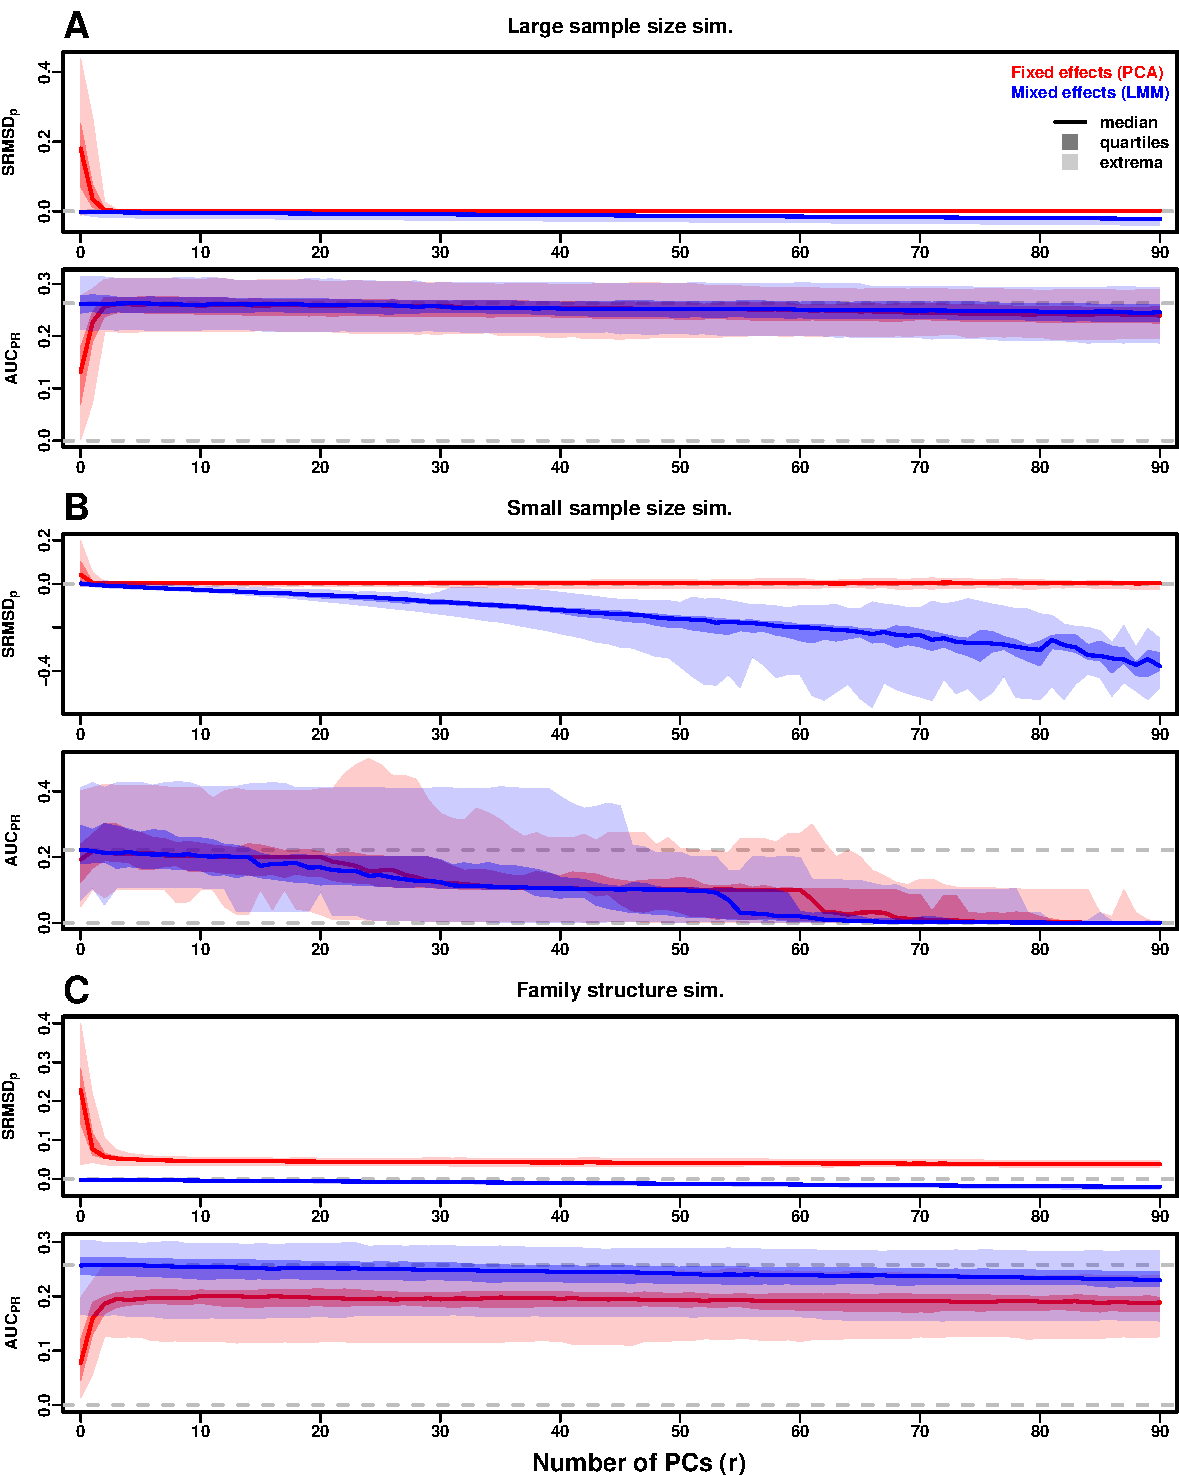
\includegraphics[width=\textwidth,height=\textheight,keepaspectratio]{rmsd-auc-sim.pdf}
  \caption{
    {\small 
      {\bf Evaluations in admixture simulations.}
      Traits simulated from \textit{random coefficients} model, otherwise the same as \cref{fig:rmsd-auc-sim}.
    }
  }
  \label{fig:rmsd-auc-sim-rc}
\end{figure}

\begin{figure}[bp!]
  \centering
  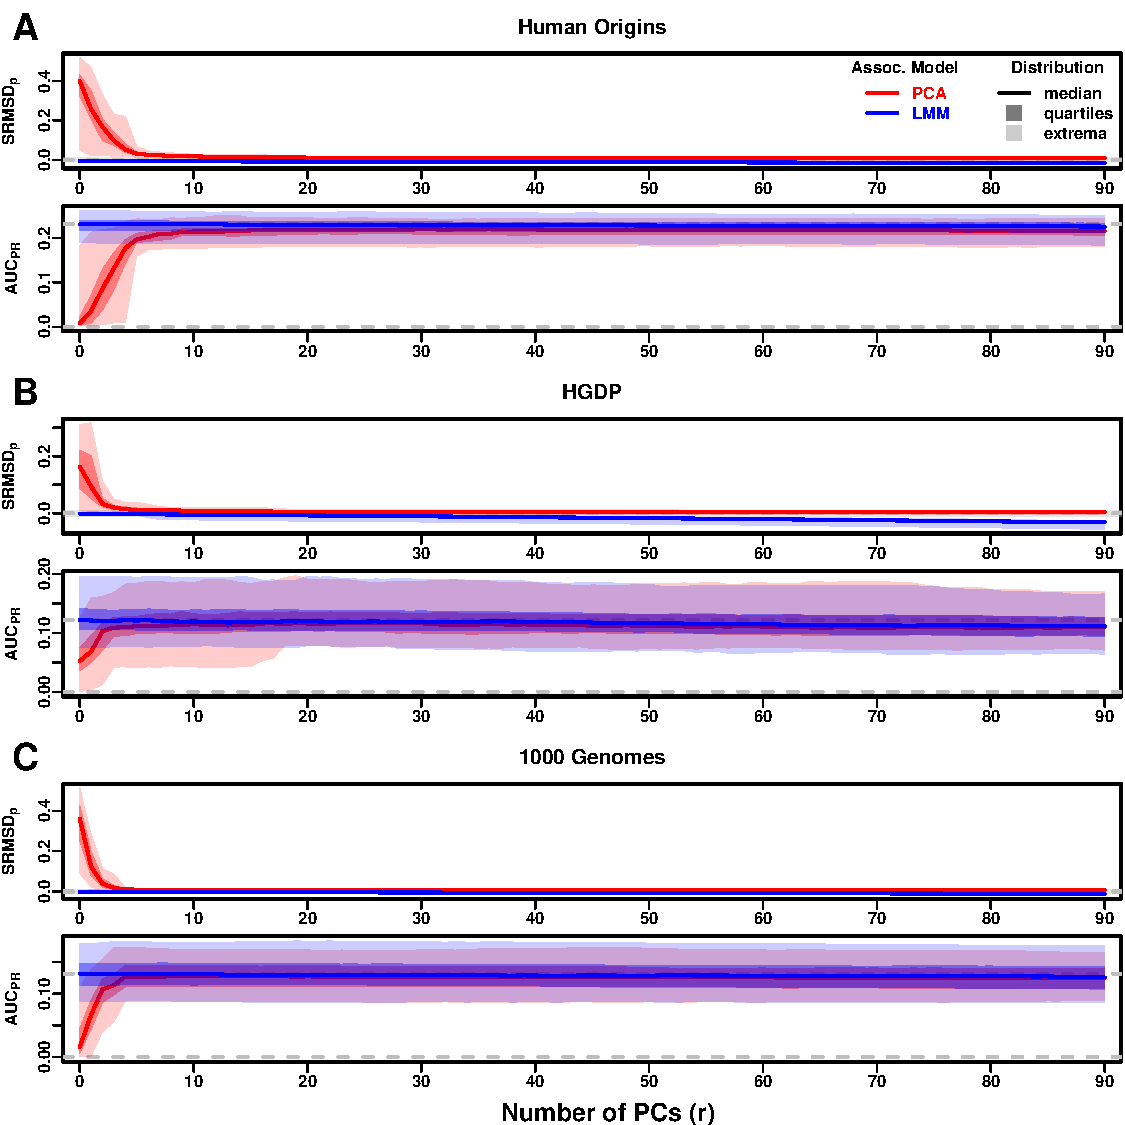
\includegraphics[width=\textwidth,height=\textheight,keepaspectratio]{rmsd-auc-real.pdf}
  \caption{
    {\small 
      {\bf Evaluations in real human genotype datasets.}
      Traits simulated from \textit{random coefficients} model, otherwise the same as \cref{fig:rmsd-auc-real}.
    }
  }
  \label{fig:rmsd-auc-real-rc}
\end{figure}

\begin{figure}[bp!]
  \centering
  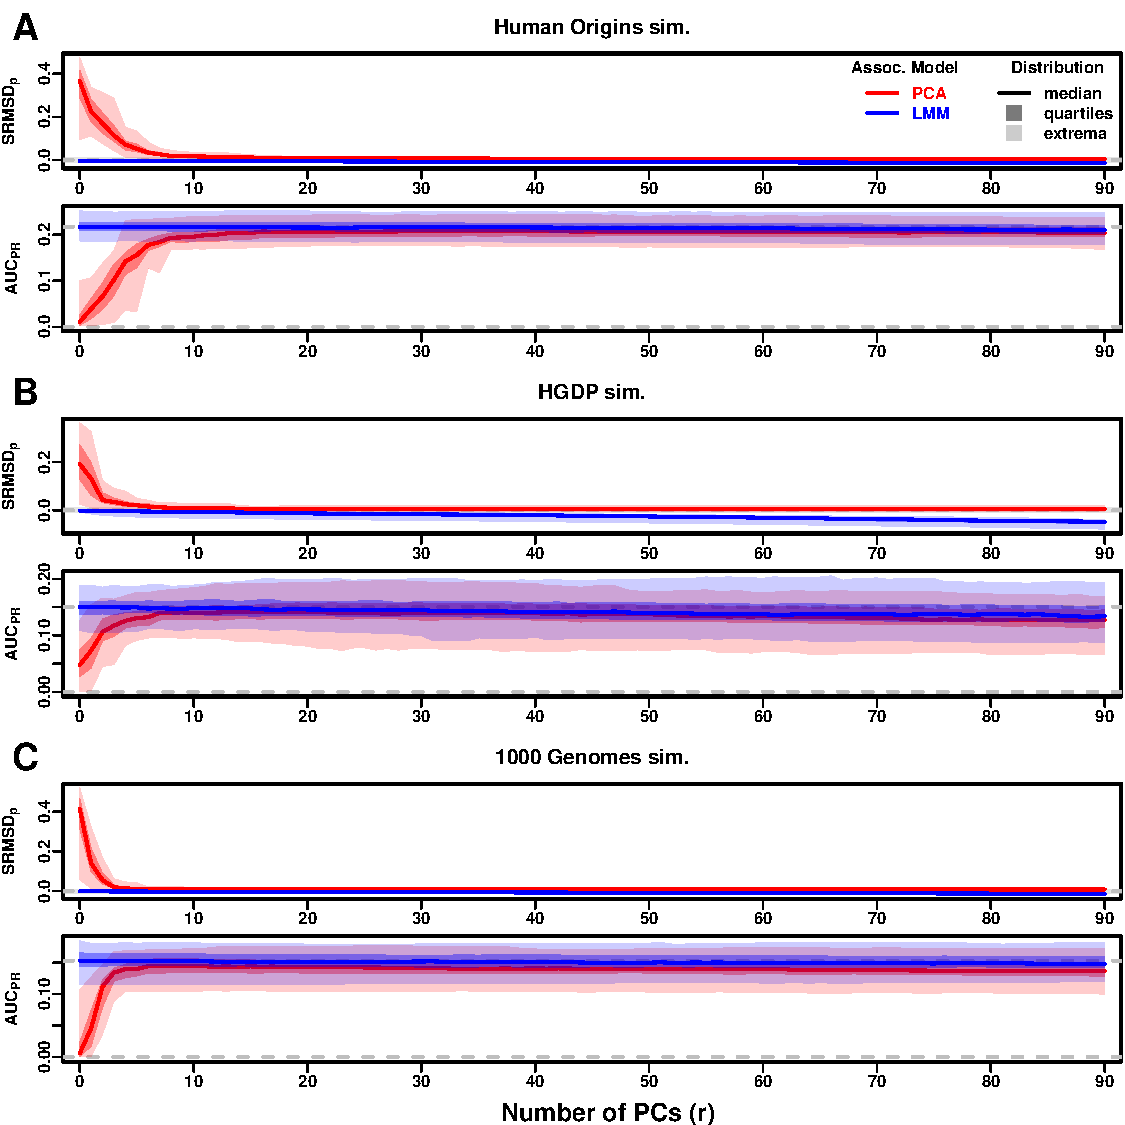
\includegraphics[width=\textwidth,height=\textheight,keepaspectratio]{rmsd-auc-real-sim.pdf}
  \caption{
    {\small 
      {\bf Evaluations in tree simulations fit to human data.}
      Traits simulated from \textit{random coefficients} model, otherwise the same as \cref{fig:rmsd-auc-real-sim}.
    }
  }
  \label{fig:rmsd-auc-real-sim-rc}
\end{figure}

\begin{figure}[bp!]
  \centering
  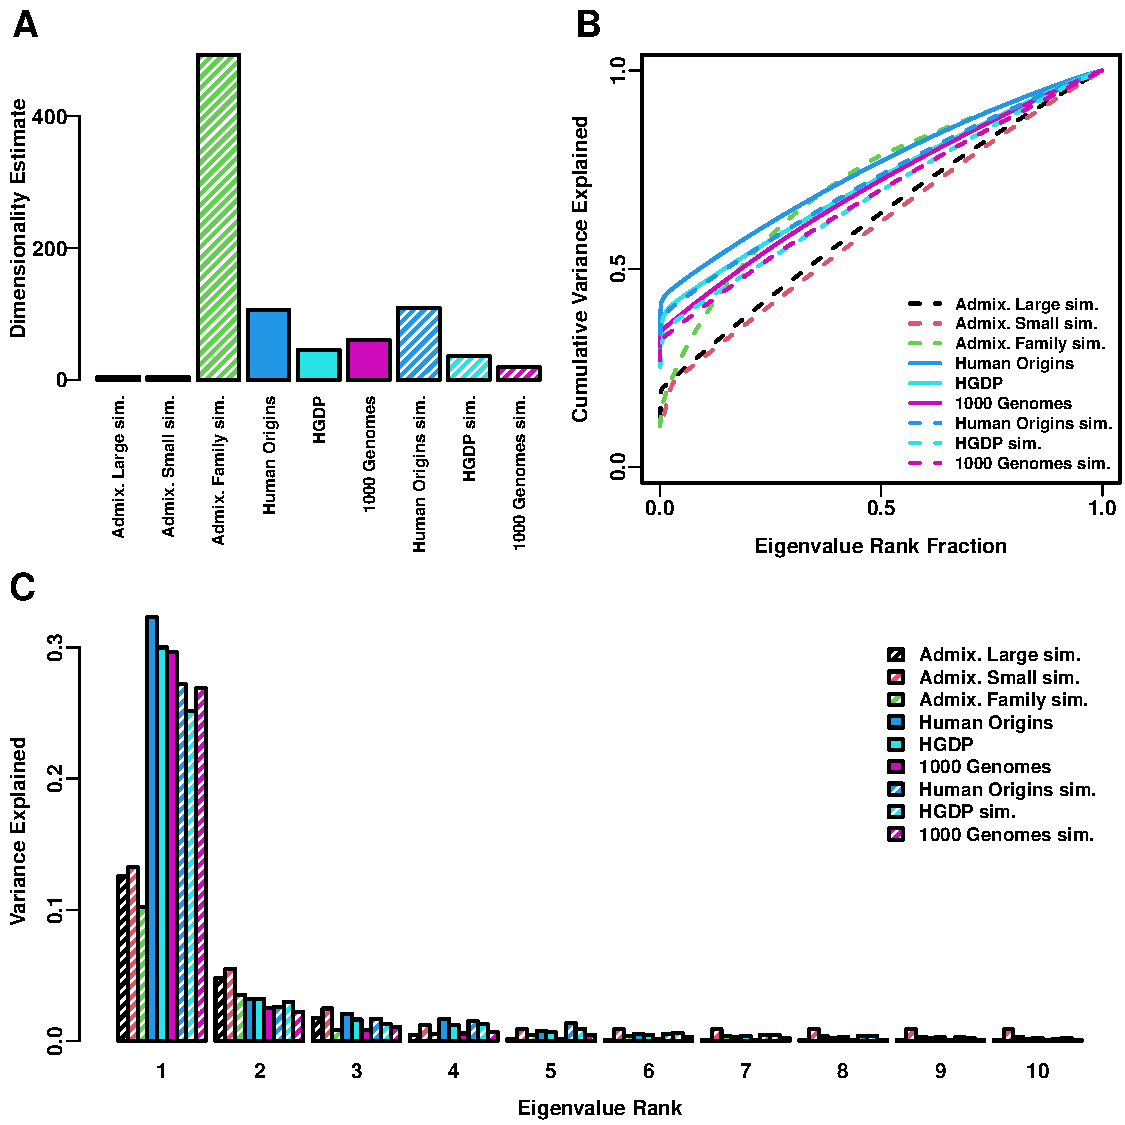
\includegraphics[width=\textwidth]{eigen.pdf}
  \caption{
    {\bf Estimated dimensionality of datasets.}
    \textbf{A.}
    Kinship matrix ranks estimated with the Tracy-Widom test with $p < 0.01$.
    \textbf{B.}
    Cumulative variance explained versus eigenvalue rank fraction ($i/n$ where $i$ is rank, $n$ is number of eigenvalues).
    \textbf{C.}
    Variance explained by first 10 eigenvalues.
  }
  \label{fig:eigen}
\end{figure}

\begin{figure}[bp!]
  \centering
  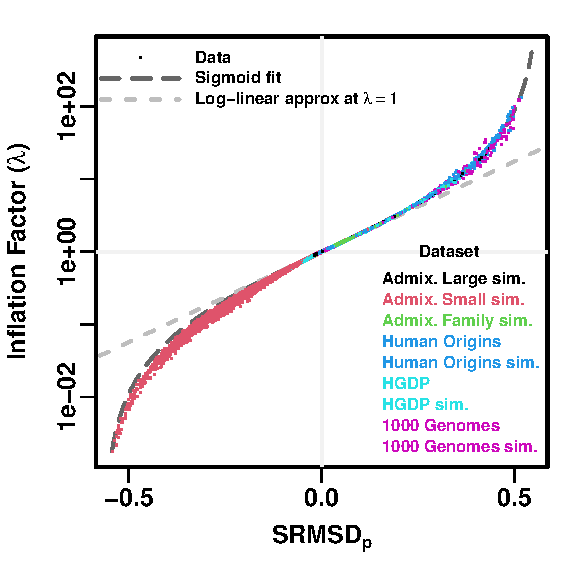
\includegraphics{sum-rmsd-vs-lambda.pdf}
  \caption{
    {\bf Comparison between $\rmsd$ and inflation factor.}
    Each point is a pair of statistics for one replicate evaluation for one association model (PCA or LMM with some number of PCs $r$), one trait model (FES vs RC), and one dataset (color coded by dataset).
    Note y-axis ($\lambda$) is on a log scale, while x-axis ($\rmsd$) is linear scale.
    The sigmoidal curve is \cref{eq:rmsd_lambda_sigmoidal} fit to the data.
  }
  \label{fig:rmsd_lambda}
\end{figure}

\clearpage

\section{Supplementary tables}

\begin{table}[hb!]
  \centering
  \footnotesize
  \caption{
    \textbf{Dataset sizes after 4th degree relative filter.}
  }
  \label{tab:king_cutoff}
  % read and automatically format data from a TSV file!
  \sisetup{ table-format = 2, table-number-alignment = right }
  \csvreader[
  tabular = {lSSS},
  separator = tab,
  table head = \toprule Dataset & {Loci ($m$)} & {Ind.~($n$)} & {Ind. removed (\%)} \\\midrule,
  late after last line = \\\bottomrule
  ]{../data/dimensions_king-cutoff-4.txt}{}{\csvlinetotablerow}
\end{table}


\end{document}